\documentclass[a4paper,12pt]{article}
\usepackage{fullpage} % Package to use full page
\usepackage[utf8]{inputenc}
%\setlength\parindent{0pt}
\usepackage{amsmath} %for writing text in equations with \text{}
\usepackage{dsfont} %for identity matrix
\usepackage[T1]{fontenc}
\usepackage{slashed}
\usepackage{tikz}
\usepackage{gensymb}
\usepackage{wrapfig}
\usepackage{subfig}

\newcommand{\icol}[1]{% inline column vector
  \left(\begin{smallmatrix}#1\end{smallmatrix}\right)%
}

\newcommand{\irow}[1]{% inline row vector
  \begin{smallmatrix}(#1)\end{smallmatrix}%
}

\title{\textbf{Gauge Theories: Electroweak}}
\author{Lecturer: Richard Ball}
\date{\normalsize\today} % Can't work out how to make this a UK format but oh well

\begin{document}

\maketitle
\section{Introduction}
%
Imagine a world without electroweak:
\begin{itemize}
    \item Still have electromagnetism (EM), massive hadrons, atoms, gravity etc.
    \item Parity (P) and charge conjugation (C) are still good symmetries
    \item Flavour is always conserved: everything lasts forever (and always existed)
    \item No neutrinos (would be non-interacting)
\end{itemize}
%
Neutrinos were first hypothesised by Pauli (1930) to explain the missing energy in $\beta$-decay. They were first observed in 1956 (Cowan-Reines). Parity violation was first directly observed in 1956/7 (Lee-Yang-Wu).

\subsection{Chirality}
%
Define the projection operators $P_R \equiv \frac{1}{2}(1 + \gamma^5)$ and $P_L \equiv \frac{1}{2}(1 - \gamma^5)$. Recalling that $(\gamma^5)^2 = 1$ and $(\gamma^5)^\dagger = \gamma^5$, we can deduce the following properties:
\begin{itemize}
    \item $P_R^2 = P_R$,
    \item $P_L^2 = P_L$,
    \item $P_LP_R = P_RP_L = 0$,
    \item $P_R + P_L = 1$,
    \item $P_R - P_L = \gamma^5$.
\end{itemize}
% 
Any Dirac spinor can be split up into a right-handed and a left-handed component, $\psi = \psi_R + \psi_L$, using the projection operators to define $\psi_R = P_R \psi$ and $\psi_L = P_L \psi$. Since $\gamma^\mu P_L = P_R \gamma^\mu$, it follows that $\bar{\psi} P_R \equiv (\bar{\psi})_R = \bar{\psi}_L$ and $\bar{\psi} P_L \equiv (\bar{\psi})_L = \bar{\psi}_R$. So 
\begin{equation}
\begin{split}
    \bar{\psi}\psi = \bar{\psi}(\psi_R + \psi_L) &= \bar{\psi}_L\psi_R + \bar{\psi}_R\psi_L \\
    &\text{and} \\
    \bar{\psi}\gamma^\mu \psi = \bar{\psi}\gamma^\mu(\psi_R + \psi_L) &= \bar{\psi}_R\gamma^\mu\psi_R 
    \bar{\psi}_L\gamma^\mu\psi_L.
\end{split}
\end{equation}
%
The Dirac Lagrangian splits up like 
\begin{equation}
\begin{split}
\mathcal{L}_D &= \bar{\psi}(i\slashed{\partial}-m)\psi \\ 
&= \bar{\psi}_R i\slashed{\partial}\psi_R + \bar{\psi}_L i\slashed{\partial}\psi_L
+ m(\bar{\psi}_L\psi_R + \bar{\psi_R}\psi_L),
\end{split}
\end{equation}
so the mass term mixes $\psi_R$ and $\psi_L$: if $m \to 0$, $\psi_R$ and $\psi_L$ are independent. In this scenario they are both 2-component spinors obeying the Weyl equation $i\slashed{\partial}\psi_{R/L} = 0$.

\subsection{Helicity}
The spin operator can be expressed as $\Sigma^i = \frac{i}{2} \epsilon^{ijk}[\gamma^j, \gamma^k] = \gamma^5\gamma^0\gamma^i$. Then $[P_L, \Sigma^i] = [P_R, \Sigma^i]$: spin and chirality commute. Now consider \textit{helicity}, defined 
\begin{equation}
    h \equiv \frac{2\underline{\Sigma} \cdot \underline{p}}{|\underline{p}|}.
\end{equation}
$h$ has eigenvalues $\pm1$, which follows from $(\slashed{p} - m)u^\pm = 0 \implies hu^\pm = \pm u^\pm$. But $\slashed{p} = E\gamma^0 - \underline{\gamma}\cdot\underline{p}$ and $h = \gamma^5\gamma^0 (\underline{\gamma}\cdot\underline{p})/|\underline{p}| = \gamma^5\gamma^0(E\gamma^0 - \slashed{p})$. So
%
\begin{equation}
\begin{split}
\gamma^5(E - \gamma^0\slashed{p})u^\pm &= \pm u^\pm \\
\implies (P_R-P_L)(E-\gamma^0m)u^\pm &= \pm p(P_R + P_L)u^\pm \\
\text{ and } (E \mp p)u_R^\pm &= m\gamma^0 u_L^\pm, \\
             (E \pm p)u_L^\pm &= m\gamma^0 u_R^\pm. 
\end{split}
\end{equation}
Again, the mass term mixes R and L, but if $m \to 0$, $p = E + \mathcal{O}(\frac{m^2}{E})$ and $2E u_R^- = 2E u_L^+ = 0$ so $u_R^- = u_L^+ = 0$, i.e. $u_R$ has helicity +1 and $u_L$ has helicity -1. 

Note that when $m=0$, helicity is Lorentz invariant (no rest frame). For $m \neq 0$, 
\begin{equation}
\begin{split}
    u_R^- = \frac{m\gamma^0}{E+p}u_L^- &\approx \frac{m}{2E}\gamma^0u_L^- \\
    \text{ and } u_L^+ &\approx \frac{m}{2E}\gamma^0u_R^+.
\end{split}
\end{equation}
You get similar expressions for negative energy solutions:
\begin{equation}
\begin{split}
\text{for $m = 0$:   } &v_R^- = v_L^+ = 0, \\
\text{for $m \neq 0$:    }  &v_R^- = -\frac{m\gamma^0}{2E}v_L^- \text{ and } v_L^+ = -\frac{m\gamma^0}{2E}v_R^-.
\end{split}
\end{equation}
%
\subsection{The Chiral Representation}
%
In the chiral representation the gamma matrices can be expressed as:
\[ \gamma^0 = \left( \begin{array}{cc}
0 & 1  \\
1 & 0  \end{array} \right), \qquad
\gamma^i = \left( \begin{array}{cc}
0 & -\sigma^i  \\
\sigma^i & 0  \end{array} \right), \qquad
\gamma^5 = \left( \begin{array}{cc}
1 & 0 \\
0 & -1     \end{array} \right).\] 
%
So
%
\[ P_R = \left( \begin{array}{cc}
1 & 0  \\
0 & 0  \end{array} \right), \qquad
P_L = \left( \begin{array}{cc}
0 & 0  \\
0 & 1  \end{array} \right) \qquad
\implies
\psi = \left( \begin{array}{c}
\psi_R  \\
\psi_L      \end{array} \right).\] 
%
Furthermore, the spin operator can be written
%
\[ \Sigma^i = \gamma^5\gamma^0\gamma^i = \left( \begin{array}{cc}
\sigma^i & 0  \\
0 & \sigma^i  \end{array} \right), \]
%
so the helicity eigenstates are $\icol{\psi_R^\pm\\0}$ and $\icol{0\\\psi_L^\pm}$. Now consider the positive and negative energy solutions. 
%
$(\slashed{p} - m)u =0 \implies$
%
\[ \left( \begin{array}{cc}
-m & E +\underline{\sigma}\cdot\underline{p}  \\
  E -\underline{\sigma}\cdot\underline{p}& -m  \end{array} \right)
\left( \begin{array}{c}
u_R   \\
u_L  \end{array} \right) = 0.\] 
%
But $\underline{\sigma}\cdot \underline{p}\ u_{L/R} = \pm p\ u_{L/R}^\pm$ so $(E \pm p)u_L^\pm = m\ u_R^\pm$. Using $E^2 = p^2 + m^2$:
\begin{equation}
\begin{split}
(E \pm p)u_L^\pm &= \sqrt{(E+p)(E-p)}u_R^\pm \\
\implies \sqrt{E\pm p}\ u_L^\pm &= \sqrt{E \mp p}\ u_R^\pm 
\end{split}
\end{equation}
and we can write
%
\[ u^\pm =
\left( \begin{array}{c}
\sqrt{E \pm p} \ \xi^\pm   \\
\sqrt{E \mp p} \ \xi^\pm  \end{array} \right), \] 
%
where $\xi^+ = \icol{1\\0}$ and $\xi^- = \icol{0\\1}$. 
\newline
\newline
\textit{Exercise: check that the normalisations $\bar{u}u = 2m$, $u^\dagger u = 2E$.}
\newline

Similarly, $(\slashed{p} +m)v = 0$ and $(\underline{\sigma}\cdot\underline{p})v^\pm = \mp p\ v^\pm$, so 
\begin{equation}
\begin{split}
(E \mp p)v_L^\pm &= -m\ v_R^\pm \\
\implies \sqrt{E\mp p}\ v_L^\pm &= -\sqrt{E \pm p}\ v_R^\pm 
\end{split}
\end{equation}
and
%
\[ v^\pm =
\left( \begin{array}{c}
\sqrt{E \mp p} \ \xi^\pm   \\
-\sqrt{E \pm p} \ \xi^\pm  \end{array} \right). \] 
%
You can relate $\xi^\pm$ to $\chi^\pm$ by charge conjugation: $v^\pm = i \gamma^2 u^{\pm *}$, where
%
\[ i\gamma^2 = \left( \begin{array}{cc}
0 & -i \sigma^2  \\
i\sigma^2 & 0  \end{array} \right), \qquad 
-i\sigma^2 = \left( \begin{array}{cc}
0 & -1 \\
1 & 0 \end{array} \right). \]
%
So $\chi^\pm = -i\sigma^2\xi^\pm$ and if $\xi^\pm = \icol{1\\0}, \icol{0\\1}$ then $\chi^\pm = \icol{0\\1}, \icol{-1\\0}$ as before.
%
\subsection{Parity}
%
Under P, $\psi \to \psi_p = \gamma^0\psi$. We know that $P_L \gamma^0 = \gamma^0 P_R$, so $\psi_L \to \gamma^0 \psi_L =  P_R\gamma^0 \psi_L = (\psi_p)_R$. In other words, $(\psi_L)_p = (\psi_p)_R$, so parity switches L and R.

Note that $[\gamma^0, \Sigma^i] = 0$ but under P $\underline{p} \to - \underline{p}$ so $h \to -h$, as expected. This means $u_R^+ to u_L^-$ etc.: parity flips helicity but not spin.
%
\subsection{Charge conjugation}
%
Under C, $\psi \to \psi_c = C\overline{\psi}^T$ where $C = i\gamma^2\gamma^0$. Then $P_LC = CP_L$ so $\psi_L \to C(\overline{\psi})_L^T$. 
This means that charge conjugation leaves the chirality unchanged. Helicity is also unchanged: C just takes particles $\leftrightarrow$ antiparticles.
%
\subsection{Time reversal}
%
Under T, $\psi \to \psi_T = B\psi$ where $B = i\gamma^1\gamma^3 = -i\gamma^5C$ and $B^\dagger = B = B^{-1}$. Again, $P_LB = BP_L$ so $\psi_L \to B\psi_L$ and time reversal leaves chirality and helicity unchanged (it reverses both spin and momentum). 
%
%%%%%%%%%%%%%%%%%%%%%%%%%%%%%%%%%%%%%%%%%%%%%%%%%%%%%%%%%%%%%%%%%%%%%%%%%%%%%%%%%%%%%%%%%%%%%%%%%%%%%%%%%
\newpage
%
\section{Charged Current Electroweak}
%
\subsection{Fermi Theory (1934)}
%
Fermi theory is based on a point-like 4-fermion interaction
\begin{equation}
    G_F(\bar{n}\gamma_\mu p)(\bar{\nu}\gamma^\mu e),
\end{equation}
representing the process $n \to pe^-\bar{\nu}$, where $n$ is a neutron, $p$ is a proton, $e^-$ is an electron and $\bar{\nu}$ is an antineutrino. More generally, the interaction can be written as $G_F J_\mu^\dagger J^\mu$ where $J_\mu$ is the "weak current" and is composed of leptonic and hadronic contributions: $J_\mu = \bar{\nu}\gamma_\mu e + \bar{p}\gamma_\mu n + ...$. Note that $J_\mu$ has $\Delta Q = +1$ so $J_\mu^\dagger$ has $\Delta Q = -1$ and electric charge is conserved. 

Considering mass dimensions $[\cdot]$: $[m\psi\bar{\psi}]=+4$, $[\psi]=3/2$ and $[J_\mu] =3$ so $[G_F]=-2$. In other words, the coupling scales as 1/mass$^2$. The mass scale is $\approx$ 300 GeV, so the interaction is weak. The original Fermi interaction conserves parity (and C and CP), just like QED. This turned out to be wrong, according to theory developed by Lee and Yang (1956) and the Wu experiment in 1957. In charged current weak interactions, P and C are violated but CP is conserved. More on this later.
%
\subsection{V-A Theory}
%
Developed by Masshart, Sudarshan, Feynman, Gell-Man ... in 1958. V-A theory is based on a vector current $V_\mu$ and an axial current $A_\mu$:
\begin{equation}
\begin{split}
V_\mu &= \bar{\nu}\gamma_\mu e + \bar{p}\gamma_\mu n + ... ,\\
A_\mu &= \bar{\nu}\gamma_\mu \gamma^5 e + \bar{p}\gamma_\mu \gamma^5 n + ...,
\end{split}
\end{equation}
whose difference gives the overall current
\begin{equation}
\begin{split}
\frac{1}{2}J_\mu = \frac{1}{2}(V_\mu - A_\mu)  &= \bar{\nu}\gamma_\mu\frac{1}{2}(1-\gamma^5) e + \bar{p}\gamma_\mu\frac{1}{2}(1-\gamma^5) n + ... \\
&= \bar{\nu}_L\gamma_\mu e_L + \bar{p}_L\gamma_\mu n_L + ... .
\end{split}
\end{equation}
So the weak interactions involve \textbf{only left-handed fields}, and maximally violate P and C. In fact, under P, C and CP the currents transform in the following ways:
\begin{equation}
\begin{split}
&P: \qquad V^\mu \to V_\mu, \qquad A^\mu \to -A_\mu, \qquad (V-A)^\mu \to (V+A)_\mu. \\
&C: \qquad V^\mu \to -V^\mu, \qquad A^\mu \to A^\mu, \qquad (V-A)^\mu \to (-V-A)^\mu. \\
&CP: \qquad V^\mu \to -V_\mu, \qquad A^\mu \to -A_\mu, \qquad (V-A)^\mu \to -(V-A)_\mu. 
\end{split}
\end{equation}
So $(V-A)^{\mu \dagger}(V-A)_\mu$ is invariant under CP (and T). 

Note that that neutrinos \textbf{only} interact weakly, so $\nu_R$ does not interact at all! If neutrinos are massless, there is no need for $\nu_R$. From 1930-1998 neutrinos were always assumed to be massless: here we will assume $m_\nu=0$ so $\nu$ are always left handed and $\bar{\nu}$ are always right handed. In reality $m_\nu \leq$ 0.3 eV, which is very small.

So we have
%
\begin{equation}
\mathcal{L}_{4F} = -\frac{G_F}{\sqrt{2}} J_\mu^\dagger J^\mu,
\end{equation}
where the $\sqrt{2}$ is historical. $J_\mu = J_\mu^l + J_\mu^h$ can be split up into a leptonic and a hadronic current, each of which comprises three generations. For example, the leptonic current,
\begin{equation}
\frac{1}{2}J_\mu^l = \bar{\nu}_e\gamma_\mu e_L + \bar{\nu}_{(\mu)}\gamma_\mu \mu_L + \bar{\nu}_\tau \gamma_\mu \tau_L.
\end{equation}
Lepton number $L_e = N_{e^-} - N_{e^+} + N_{\nu_e} - N_{\bar{\nu}_e}$ and the corresponding $L_\mu$ and $L_\tau$ are conserved, according to Noether's Theorem.  

The hadronic current,
\begin{equation}
\frac{1}{2}J_\mu^h = \bar{u}_L\gamma_\mu d_L^\prime + \bar{c}_L \gamma_\mu s_L^\prime + \bar{t}_L \gamma_\mu b_L^\prime,
\end{equation}
is simplest to express in terms of the quarks. The baryon number $B = \sum_{gen} (N_u -N_{\bar{u}} + N_d - N_{\bar{d}})$ is conserved. Things are complicated due to the effects of quark mixing - see later.

(V-A) Theory is quite complicated, but there is only one coupling, $G_F$: we call this universality. Explicitly,
\begin{equation}
\mathcal{L}_{4F} = -\frac{G_F}{\sqrt{2}} (J_\mu^{l \dagger} J^{l\mu} + (J_\mu^{h \dagger} J^{l\mu} + J_\mu^{l \dagger} J^{h\mu}) + J_\mu^{h \dagger} J^{h\mu} ),
\end{equation}
so there are three types of (charged current) weak interaction:
\begin{itemize}
    \item \textbf{leptonic,} only leptons (and neutrinos) e.g. $\mu \to e \nu_\mu \bar{\nu}_e$;
    \item \textbf{semi-leptonic,} both leptons and quarks e.g. $\pi^- = d\bar{u} \to \mu^- \bar{\nu}_\mu$;
    \item \textbf{hadronic,} only quarks e.g. $\Lambda \to p \pi$.
\end{itemize}
But all of them violate P and C and conserve CP, only involve left-handed particles and only involve one coupling $G_F$. 
\newline
\newline
\subsubsection{Example: $\pi^+ \approx u\bar{d} \to \mu^+ \nu_\mu$}
Fig. \ref{pioncp} demonstrates the sequential application of C and P to this process. Neither of the intermediate steps can happen, as they involve either a right-handed neutrino or a left-handed antineutrino.
\begin{figure}[h!]
\caption{Visualisation of applying C and P to the process $\pi^+ \approx u\bar{d} \to \mu^+ \nu_\mu$.}
\label{pioncp}
\centering
\begin{tikzpicture}
\draw[<-] (0,1) -- (1,1);
\node[] at (0,0.5) {$\mu^-$};
\draw[fill=black] (1.5,1) circle (0.1cm);
\node[] at (1.5,0.5) {$\pi^-$};
\draw[->] (2,1) -- (3,1) ;
\node[] at (3, 0.5){$\bar{\nu}_\mu$};
%
\draw[<-] (-4,3) -- (-3,3);
\node[] at (-4,2.5) {$\mu^+$};
\draw[fill=black] (-2.5,3) circle (0.1cm);
\node[] at (-2.5,2.5) {$\pi^+$};
\draw[->] (-2,3) -- (-1,3) ;
\node[] at (-1, 2.5){$\nu_\mu$};
%
\draw[->] (5.5,3) -- (6.5,3);
\node[] at (6.5,2.5) {$\mu^-$};
\draw[fill=black] (5,3) circle (0.1cm);
\node[] at (5,2.5) {$\pi^-$};
\draw[->] (4.5,3) -- (3.5,3) ;
\node[] at (3.5, 2.5){$\bar{\nu}_\mu$};
%
\draw[<-] (0,6) -- (1,6);
\node[] at (0,5.5) {$\nu_\mu$};
\draw[fill=black] (1.5,6) circle (0.1cm);
\node[] at (1.5,5.5) {$\pi^-$};
\draw[->] (2,6) -- (3,6) ;
\node[] at (3, 5.5){$\mu^+$};
%
\draw[->] (1.5,5) --(1.5,2) ;
\draw[->] (2.5,5) --(4.5,4) ;
\draw[->] (0.5,5) --(-1.5,4) ;
\draw[<-] (2.5,1.5) --(4.5,2) ;
\draw[<-] (0.5,1.5) --(-1.5,2) ;
%
\node[] at (2,3.5) {CP};
\node[] at (4,5) {C};
\node[] at (-1,5) {P};
\node[] at (-1,1.5) {C};
\node[] at (4,1.5) {P};
%
\draw[red,->] (2.5,1.25) -- (3,1.25);
\draw[red,->] (0,6.25) -- (0.5,6.25);
\draw[red,->] (-1.5,3.25) -- (-1,3.25);
\draw[red,->] (3.5,3.25) -- (4,3.25);
\end{tikzpicture}
\end{figure}
%
\subsection{Leptonic decays}
%
\subsubsection{Example: $\mu^- \to e^- \bar{\nu}_e \nu_\mu$}
\begin{wrapfigure}{l}{0.4\linewidth}
  \centering
  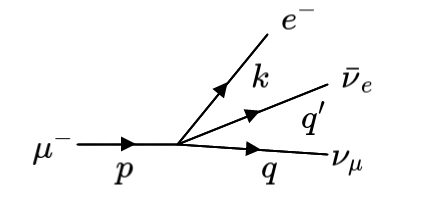
\includegraphics[width=\linewidth]{figs/diag_1.png}
\end{wrapfigure}
We will work with Dirac spinors everywhere and contract the spiniors as required.
The matrix element can be written
\begin{equation}
  \mathcal{M} = \langle e^-(k);\bar{\nu}_e(q^\prime)|\mathcal{L}_{4F}|\mu^-(p) \rangle,
\end{equation}
and we can identify the Feynman rule for the four fermion vertex as 
\begin{equation}
  -i\frac{G_F}{\sqrt{2}} [\gamma_\mu(1-\gamma^5)]_{ab} [\gamma^\mu(1-\gamma^5)]_{cd}
\end{equation}
so 
\begin{equation}
  \mathcal{M} = -i\frac{G_F}{\sqrt{2}} \bigg(\bar{u}(k)\gamma^\mu(1-\gamma^5)v(q^\prime)\bigg) \bigg(\bar{u}(q)\gamma_\mu(1-\gamma^5)u(p)\bigg),
\end{equation}
where $\bar{u}(k)$, $v(q^\prime)$, $\bar{u}(q)$ and $u(p)$ refer to the electron, anti-electron neutrino, muon neutrino and muon respectively. 

Average over initial spins and sum over final spins (assuming the neutrinos are massless):
\begin{equation}
    \frac{1}{2} \sum_{spins} |\mathcal{M}|^2 = \frac{1}{4}G_F^2\ tr\bigg((\slashed{k}+m_e)\gamma^\mu(1-\gamma^5)\slashed{q}^\prime\gamma^\nu(1-\gamma^5)\bigg)\ tr\bigg(\slashed{q}\gamma_\mu(1-\gamma^5)(\slashed{p}+m_\mu)\gamma_\nu(1-\gamma^5)\bigg),
\end{equation}
where we call the first trace $\mathcal{M}^{\mu \nu}(k,q^\prime)$ and the second trace $\mathcal{M}_{\mu \nu}(q,p)$. Consider evaluating one of these traces, using $(1-\gamma^5)^2 = 2(1-\gamma^5)$ and $tr\gamma^5\gamma^\mu \gamma^\nu \gamma^\alpha \gamma^\beta = 4i\epsilon^{\mu \nu \alpha \beta}$:
\begin{equation}
\begin{split}
    \mathcal{M}_{\mu \nu}(q,p) &= 2\ tr\bigg( \slashed{q}\gamma_\mu(\slashed{p} + m_\mu)\gamma_\nu(1-\gamma^5)\bigg)\\
    &= 8(q_\mu p_\nu + p_\mu q_\nu - \eta_{\mu \nu} p \cdot q - i \epsilon_{\alpha \mu \beta \nu} q^\alpha p^\beta) \\
    &= 8(q_\mu p_\nu + p_\mu q_\nu - \eta_{\mu \nu} p \cdot q + i \epsilon_{\mu \nu \alpha \beta} q^\alpha p^\beta),
\end{split}
\end{equation}
so
\begin{equation}
\begin{split}
\frac{1}{2}\sum_{spins}|\mathcal{M}|^2 &= 16\ G_F^2(k^\mu q^{\prime \nu} + q^{\prime \mu} k^\nu - \eta^{\mu \nu} k \cdot q^\prime - i \epsilon^{\mu \nu \alpha \beta} q^{\prime \alpha} k_\beta)(q_\mu p_\nu + p_\mu q_\nu - \eta_{\mu \nu} p \cdot q + i \epsilon_{\mu \nu \rho \sigma} q^\rho p^\sigma) \\
&= 16\ G_F^2(2p\cdot k q \cdot q^\prime + 2 p \cdot q^\prime k \cdot q + 4 p \cdot q k \cdot q^\prime - 4 k \cdot q^\prime p \cdot q + \epsilon^{\mu \nu \alpha \beta} \epsilon_{\mu \nu \rho \sigma} q^\prime_\alpha k_\beta q^\rho p^\sigma) \\
&= 64\ G_F^2 p \cdot q^\prime k \cdot q.
\end{split}
\end{equation}
Now we want to evaluate the decay rate in the lab frame of the muon. Here $E(p) = m_\mu$.
\begin{equation}
\begin{split}
d\Gamma &= \frac{1}{2m_\mu}\frac{1}{2}\sum_{spins}|\mathcal{M}|^2(dPS)_3 \\
& = \frac{1}{2m_\mu} \int \frac{d^3k}{(2\pi)^3 2k^0}\frac{d^3q}{(2\pi)^3 2q^0}\frac{d^3q^\prime}{(2\pi)^3 2q^{\prime 0}}(2\pi)^4\delta^4(p-k-q-q^\prime)\frac{1}{2}\sum_{spins}|\mathcal{M}|^2 \\
&= \frac{G_F^2}{8 m_\mu \pi^5} \int \frac{d^3k}{k^0} \frac{d^3q}{q^0} \frac{d^3q^\prime}{q^{\prime 0}} \delta^4(p-k-q-q^\prime)(p \cdot q^\prime)(k \cdot q).
\end{split}
\end{equation}
Integrate over $q$ and $q^\prime$, since these are unobserved. Write $Q = q + q^\prime = p - k$, $Q^2 = 2 q \cdot q^\prime = 2(q^0 q^{\prime 0} -\underline{q}\cdot \underline{q}^\prime) \geq 0$. Then we need to evaluate the integral
\begin{equation}
	\mathcal{I}_{\mu \nu}(Q) \equiv \int \frac{d^3q}{q^0} \frac{d^3 q^\prime}{q^{\prime 0}} \delta^4(Q - q - q^\prime) q_\mu q^\prime_\nu.
\end{equation}
Appealing to Lorentz invariance, we can write $\mathcal{I}_{\mu \nu} = a Q_\mu Q_\nu + b \eta_{\mu \nu} Q^2$ for some $a$, $b$ to be found. This is because these are the only two Lorentz invariant terms which can be constructed using the vectors and tensors available. In order to find the coefficients $a$ and $b$, we can systematically contract the expression with $\eta^{\mu \nu}$ and $Q^\mu Q^\nu$. This gives
\begin{equation}
\begin{split}
a + 4b &= \frac{1}{2}\mathcal{I}, \\
a + b &= \frac{1}{4}\mathcal{I}, \\
\text{where } \mathcal{I} &= \int \frac{d^3q}{|q|} \frac{d^3 q^\prime}{|q^\prime|} \delta^4(Q - q - q^\prime)
\end{split}
\end{equation}
and we have used $q^0 = |q|$, $Q \cdot q Q \cdot q^\prime = (q \cdot q^\prime)^2 = 1/4\ Q^4$. Since $\mathcal{I}$ is a Lorentz scalar, we can evaluate it in any frame. Choose $Q^\mu = (Q^0, \underline{0})$, where $\underline{q} = - \underline{q^\prime}$.
\begin{equation}
\begin{split}
\mathcal{I} &= \int \frac{d^3\underline{q}}{|\underline{q}|^2}\ \delta(Q^0 - 2 |\underline{q}|) \\
&= 4 \pi \int_0^\infty dq\ \delta(Q^0 - 2q) \\
&= 2 \pi,
\end{split}
\end{equation}
so $a = \pi /3$ and $b= \pi /6$. Putting everything together,
\begin{equation}
p^\mu k^\nu \mathcal{I}_{\mu \nu}(Q) = \frac{1}{6} \pi (2 Q \cdot p Q \cdot k + p \cdot k Q^2),
\end{equation}
so 
\begin{equation}
\begin{split}
    d\Gamma &= \frac{G_F^2}{3 m_\mu (2\pi)^4)} \int \frac{d^3\underline{k}}{k^0}\ \bigg(2p \cdot (p-k) k \cdot (p-k) + p \cdot k (p-k)^2\bigg) \\
    &= \frac{G_F^2}{3 m_\mu (2\pi)^4)}  \int \frac{d^3\underline{k}}{k^0}\ \bigg(-2p^2k^2 + 3(p^2+k^2)p \cdot k -4(p \cdot k)^2\bigg).
\end{split}
\end{equation}
In the muon rest frame, $p \cdot k = m_\mu E$, where $E \equiv k^0$, and $\frac{d^3\underline{k}}{k^0} \to 4\pi |\underline{k}|dE$. We can ignore $m_e \ll m_\mu$. Then
\begin{equation}
    d\Gamma = \frac{2G_F^2}{3(2\pi)^3} m_\mu E^2(3m_\mu - 4E)dE,
\end{equation}
but $Q^2 > 0$ so $m_\mu^2 - 2p\cdot k = m_\mu(m_\mu - 2e) >0$, i.e. $E < m_\mu/2$. The total cross-section
\begin{equation}
\begin{split}
    \Gamma &= \frac{G_F^2}{12\pi^3} m_\mu \int_0^{m_\mu/2} dE (3m_\mu E^2 - 4E^3) \\
    &= \frac{G_F^2 m_\mu^5}{192 \pi^3}.
\end{split}
\end{equation}
We can then use this to determine $G_F$: $\tau_\mu$ = 2.2$\times 10^{-6}$s and $\Gamma_\mu$ = 3.0$\times 10^{-19}$GeV, so $G_F \approx 1.2\times 10^{-5}$GeV$^{-2}$. 

You can use the same expression for $\tau^- \to \mu^- \bar{\nu}_\mu \nu_\tau$, $e^- \bar{\nu}_e \nu_\tau$ as a nice test of universality: $\Gamma(\tau^- \to \mu^- \bar{\nu}_\mu \nu_\tau) = \Gamma(\tau^- \to e^- \bar{\nu}_e \nu_\tau) = B\ \Gamma_\tau = (\frac{m_\tau}{m_\mu})^5\ \Gamma_\mu \approx 4 \times 10^{-13}$GeV.

\subsection{Semi-leptonic decays}
\subsubsection{Example:  $\pi^+ \to \mu^+ \nu_\mu$}
\begin{wrapfigure}{l}{0.4\linewidth}
  \centering
  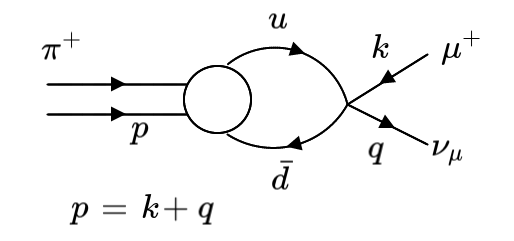
\includegraphics[width=\linewidth]{figs/diag_2.png}
\end{wrapfigure}
The matrix element can be written 
\begin{equation}
\begin{split}
    \mathcal{M} &= \langle \mu^+(k) \nu_\mu(q) | \mathcal{L}_{4F} | \pi^+(p) \rangle \\
    &= \frac{-iG_F}{\sqrt{2}} \bar{u}(q)\gamma^\mu(1-\gamma^5)v(k) \langle 0 | \bar{d}\gamma_\mu(1-\gamma^5)u | \pi^+(p) \rangle,
\end{split}
\end{equation}
in other words, it factorises into a lepton piece and a quark piece, where the quark piece is of $V_\mu - A_\mu$ form. The pion is a pseudoscalar, so $\langle 0 | V_\mu | \pi^+ \rangle = 0$. The $\langle 0 | A_\mu | \pi^+ \rangle$ piece is a four-vector, so Lorentz invariance means it must take the form $\langle 0 | A_\mu | \pi^+ \rangle = i f_\pi p_\mu$, with $f_\pi$ some "pion decay constant" to be found. This means we can write
\begin{equation}
    \mathcal{M} = \frac{G_F f_\pi}{\sqrt{2}}\bar{u}(q)\slashed{p}(1-\gamma^5)v(k).
\end{equation}
But $p = k + q$, and using $\slashed{q}u(q)=0$; $(\slashed{k} + m_\mu)v(k)=0$ gives $\bar{u}(q)(\slashed{k} + \slashed{q})(1-\gamma^5)v(k) = -m_\mu \bar{u}(q)(1+ \gamma^5) v(k)$. Now we would like to evaluate the spin-averaged matrix element squared, taking note that $(1+\gamma^5)m_\mu(1-\gamma^5)=0$:
\begin{equation}
\begin{split}
\sum_{spins}|\mathcal{M}|^2 &= \frac{G_F^2}{2} f_\pi^2 m_\mu^2 tr\ \slashed{q}(1+\gamma^5) \slashed{k} (1-\gamma^5) \\
&= 4G_F^2 f_\pi^2 m_\mu^2\ k \cdot q \\
&= 2G_F^2 f_\pi^2 m_\mu^2(m_\pi^2 - m_\mu^2).
\end{split}
\end{equation}
In the lab frame,
\begin{equation}
    d\Gamma = \frac{1}{2m_\mu} \sum_{spins} |\mathcal{M}|^2(dPS)_2,
\end{equation}
while
\begin{equation}
\begin{split}
\int(dPS)_2 &= \frac{1}{(4\pi)^2} \frac{|\underline{k}|}{m_\pi} \int d\Omega \\
&= \frac{1}{4\pi}\frac{|\underline{k}|}{m_\pi},
\end{split}
\end{equation}
where $|\underline{k}| = (m_\pi^2 - m_\mu^2)/2m_\pi$. So
\begin{equation}
\Gamma = \frac{1}{8\pi} G_F^2f_\pi^2 \frac{m_\mu^2}{m_\pi^3}(m_\pi^2 - m_\mu^2)^2.
\end{equation}
Using the measured rate for $\tau = 2.6 \times 10^{-8}$s, we can calculate $f_\pi \approx 130$ MeV. Note that 
\begin{equation}
\frac{\Gamma(\pi \to e \nu_e)}{\Gamma(\pi \to \mu \nu_\mu)} = \frac{m_e^2}{m_\mu^2}\frac{(m_\pi^2 - m_e^2)^2}{(m_\pi^2 - m_\mu^2)^2} \approx 10^{-4}.
\end{equation}
This is a good test of lepton universality. The ratio vanishes as $m_e \to 0$: this is because of helicity conservation. 
%
\subsection{Cabibbo mixing (1963)}
The Kaon decay $K^+ (u\bar{s}) \to \mu^+ \nu_\mu$ works similarly: $\langle 0 | A_\mu | K^+(p) \rangle = i f_k p_\mu$, and from experiment
\begin{equation}
    \frac{\Gamma(K \to \mu\nu)}{\Gamma(\pi \to \mu\nu)} \approx 1.3. 
\end{equation}
But if $\mathcal{L}_{4F}$ contained $\bar{u}_L \gamma_\mu s_L$ (in an analogy with $\bar{u}_L \gamma_\mu d_L$) we expect
\begin{equation}
    \frac{\Gamma(K \to \mu\nu)}{\Gamma(\pi \to \mu\nu)} = \frac{f_K^2}{f_\pi^2}\frac{m_\pi^3}{m_K^3}\frac{(m_K^2 - m_\mu^2)^2}{(m_\pi^2 - m_\mu^2)^2} \approx 24,
\end{equation}
since $f_K/f_\pi \approx 1.2$, i.e. SU(3) symmetry breaking is small.

The explanation is down to the form of the hadronic weak current. In actual fact this is
\begin{equation}
 \frac{1}{2}J_\mu^h = \bar{u}_L\gamma_\mu(\cos\theta_c\ d_L + \sin\theta_c\ s_L) + ..., 
\end{equation}
where the term in brackets can be thought of as $d_L^\prime$, a \textit{mixture} of $d$ and $s$. Then 
\begin{equation}
    \Gamma(\pi \to \mu\nu) = \frac{G_F^2}{4\pi} f_\pi^2 \frac{m_\mu^2}{m_\pi^3}(m_\pi^2 - m_\mu^2)^2 \cos^2\theta_c
\end{equation} 
and
\begin{equation}
    \Gamma(K \to \mu\nu) = \frac{G_F^2}{4\pi} f_K^2 \frac{m_\mu^2}{m_K^3}(m_K^2 - m_\mu^2)^2 \sin^2\theta_c.
\end{equation} 
The Cabibbo angle, $\theta_c \approx 13\degree$, so $\cos\theta_c = 0.97$ and $\sin\theta_c = 0.22$. This reduces the relative size of $\Gamma(K \to \mu\nu)$ by a factor of roughly 20. We will revisit quark mixing later - stay tuned!
%
\subsection{Beta decay}
$n \to p\ e^- \bar{\nu}_e$.
\newline

\begin{wrapfigure}{l}{0.4\linewidth}
  \centering
  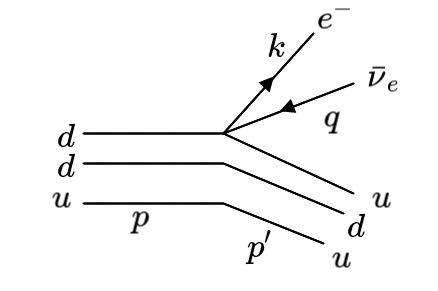
\includegraphics[width=\linewidth]{figs/diag_3.png}
\end{wrapfigure}
What's really going on is $d \to u\ e^- \bar{\nu}_e$: the other quarks are "spectators". Again, the matrix element factorises:
\begin{equation}
\begin{split}
    \mathcal{M} &= \langle p(p^\prime) e^-(k)\bar{\nu}_e(q) | \mathcal{L}_{4F} | n(p) \rangle \\
    &= \frac{-iG_F}{\sqrt{2}} \bar{u}(k)\gamma^\mu(1-\gamma^5)v(q)\\
    &\times \langle p(p^\prime) | \bar{d}^\prime\gamma_\mu(1-\gamma^5)u | n(p) \rangle \cos\theta_c.
\end{split}
\end{equation}
Considering the hadronic part,
\begin{equation}
\langle p(p^\prime) | (V_\mu - A_\mu) | n(p) \rangle = \cos\theta_c\bar{u}(p^\prime)\gamma_\mu(g_V-g_A\gamma^5)u(p),
\end{equation}
where $g_V =1$ and $g_A = 1.25$. Then 
\begin{equation}
\begin{split}
\frac{1}{2}\sum_{spins}|\mathcal{M}|^2 &= \frac{1}{4}G_F^2\cos^2\theta_c\ tr\bigg((\slashed{k} + m_e)\gamma^\mu(1-\gamma^5)\slashed{q}\gamma^\mu(1-\gamma^5)\bigg)\\
&\times tr\bigg((\slashed{p}^\prime + m_p) \gamma_\mu(1-g_A\gamma^5)(\slashed{p}+m_n)\gamma_\nu(1-g_A\gamma^5)\bigg) \\
&= \frac{1}{4}G_F^2\cos^2\theta_c\ \mathcal{M}^{\mu\nu}(k,q)\tilde{\mathcal{M}}_{\mu\nu}(p^\prime,p).
\end{split}
\end{equation}
Recalling the previous calculation for $\mu \to e\ \nu \bar{\nu}$, 
\begin{equation}
\tilde{\mathcal{M}}_{\mu\nu}(p^\prime,p) = 4\bigg((p_\mu^\prime p_\nu + p_\mu p_\nu^\prime - \eta_{\mu\nu} p \cdot p^\prime)(1+g_A^2) + i g_A \epsilon_{\mu\nu\alpha\beta}p^{\prime \alpha}p^\beta + m_n m_p(1-g_A^2)\eta_{\mu\nu}\bigg)
\end{equation}
so
\begin{equation}
\begin{split}
\frac{1}{2}\sum_{spins}|\mathcal{M}|^2 &= 8 G_F^2\cos^2\theta_c\ \bigg((2p\cdot k p^\prime \cdot q + 2 p\cdot q p^\prime \cdot k)(1+g_A)^2 \\
&- 4g_A(k\cdot p q\cdot p^\prime - k\cdot p^\prime q\cdot p) - 2 m_n m_p(1-g_A^2)k \cdot q\bigg)\\
&= 16G_F^2\cos^2\theta_c\ \bigg(p\cdot k p^\prime \cdot q (1-g_A)^2 + p\cdot q p^\prime \cdot k (1+ g_A)^2 - (1-g_A^2)m_n m_p k \cdot q \bigg).
\end{split}
\end{equation}
The decay rate
\begin{equation}
\begin{split}
d\Gamma &= \frac{1}{2m_n} \int\frac{d^3k}{(2\pi)^32k^0} \int\frac{d^3q}{(2\pi)^32q^0} \int\frac{d^3p^\prime}{(2\pi)^32p^{\prime 0}}\ (2\pi)^4 \delta^4(p - p^\prime -k - q)\frac{1}{2}\sum_{spins}|\mathcal{M}|^2 \\
&= \frac{1}{16m_n(2\pi)^5}\int\frac{d^3k}{k^0} \int\frac{d^3q}{q^0}\frac{1}{p^{\prime 0}}\ \delta(p^0 - p^{\prime 0} - k^0 - q^0) \frac{1}{2}\sum_{spins}|\mathcal{M}|^2.
\end{split}
\end{equation}
Now write $p^0 = E_p$, $p^{\prime 0} = E_p$, $k^0 = E_e$, $q^0 = E_\nu$ and $d^3k = p_e E_e\ dE_e\ d\Omega_e$, $d^3q = E_\nu^2\ dE_\nu\ d\Omega_\nu$. Using $p_e^2 = E_e^2 - m_e^2$ we can rewrite $p_e\ dp_e = E_e\ dE_e$. So
\begin{equation}
\begin{split}
    d\Gamma &= \frac{1}{16m_n(2\pi)^5}\int dE_e\ d\Omega_e\ d\Omega_\nu\ dE_\nu \bigg(\frac{p_e E_\nu}{E_p}\bigg) \delta(E_n - E_p -E_e - E_\nu) \frac{1}{2}\sum_{spins}|\mathcal{M}|^2 \\
  \implies  \frac{d\Gamma}{dE_e} &= \frac{1}{16m_n(2\pi)^5}\int d\Omega_e\ d\Omega_\nu \bigg(\frac{p_e E_\nu}{E_p}\bigg)\frac{1}{2}\sum_{spins}|\mathcal{M}|^2.\\
\end{split}
\end{equation}
Now in the lab frame, $E_n = m_n$. It is useful to define $\Delta \equiv m_n - m_p = 1.29$ MeV $\ll m_n$. We can ignore nuclear recoil by using the Born-Oppenheimer approximation, i.e. $E_p \approx m_p$. Note that $m_e=0.51$ MeV is of the same order as $\Delta$. Then 
\begin{equation}
\begin{split}
&p \cdot k p^\prime \cdot q \approx m_nE_e m_p E_\nu, \\
&p \cdot q p^\prime \cdot k \approx m_nE_\nu m_pE_e, \\
& k \cdot q = E_e E_\nu - \underline{p}_e . \underline{p}_\nu,
\end{split}
\end{equation}
so
\begin{equation}
\begin{split}
\frac{d\Gamma}{dE_e} &= \frac{G_F^2 \cos^2\theta_c}{m_n(2\pi)^5} \int d\Omega_e \ d\Omega_\nu \frac{p_e E_\nu}{E_p} m_n\ m_p\ \bigg(E_eE_\nu(1-g_A)^2 \\ &+ E_\nu E_e(1+g_A)^2 - E_e E_\nu(1-g_A^2)\bigg(1-\frac{\underline{p}_e.\underline{p}_\nu}{E_e E_\nu}\bigg)\bigg) \\
&= \frac{G_F^2\cos^2\theta_c}{2\pi^3}(1+3g_A^2)p_eE_e(\Delta-E_e)^2, \quad m_e < E_e < \Delta,
\end{split}
\end{equation}
where the $\underline{p}_e\underline{p}_\nu$ term integrates to zero. This evaluates to
\begin{equation}
\Gamma = \frac{G_F^2\cos^2\theta_c}{2\pi^3}(1+3 g_A^2) \Delta^5 \times \#
\end{equation}
where $\# = 0.47$ (left as an exercise).

Other semileptonic processes include:
\begin{equation}
\begin{split}
\Delta S = 0: \qquad &\pi^+ \to \pi^0e^+\nu; \qquad \cos\theta_c \\
\Delta S = 1: \qquad &K^+ \to \pi^0\mu^+\nu,\ K^0 \to \pi^-\mu^+\nu\ \text{etc.}; \qquad \sin\theta_c,
\end{split}
\end{equation}
and decays of the hyperons $\Sigma = uus$, $\Lambda = uds$, $\Xi = uss$, $\Omega = sss$ etc., which are all related by SU(3):
\begin{equation}
\begin{split}
\Delta S = 0: \qquad &\Sigma \to \Lambda e \bar{\nu}; \\
\Delta S = 1: \qquad &\Lambda \to pe\bar{\nu},\ \Sigma \to ne\bar{\nu}; \\
&\Xi \to \Sigma e \bar{\nu},\ \Omega \to \Xi e \bar{\nu}\ \text{etc.} 
\end{split}
\end{equation}
\subsection{Nonleptonic decays}

e.g. $K \to \pi \pi$, $K \to \pi \pi \pi$, $\Lambda \to p \pi$, $\Omega \to \Xi \pi$ etc.
\newline
%\begin{wrapfigure}{l}{0.4\linewidth}
  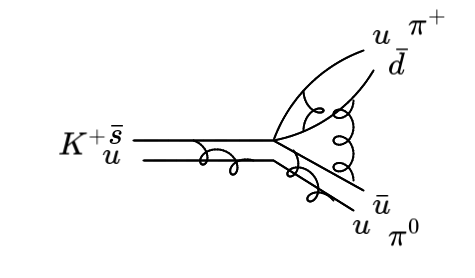
\includegraphics[width=0.5\linewidth]{figs/diag_4.png}
%\end{wrapfigure}
\newline
Here factorisation no longer holds - there are strong interactions everywhere! We need to resort to non-perturbative methods such as lattice QCD (see later in the course).
%%%%%%%%%%%%%%%%%%%%%%%%%%%%%%%%%%%%%%%%%%%%%%%%%%%%%%%%%%%%%%%%%%%%%%%%%%%%%%%%%%%%%
%%%%%%%%%%%%%%%%%%%%%%%%%%%%%%%%%%%%%%%%%%%%%%%%%%%%%%%%%%%%%%%%%%%%%%%%%%%%%%%%%%%%%
%%%%%%%%%%%%%%%%%%%%%%%%%%%%%%%%%%%%%%%%%%%%%%%%%%%%%%%%%%%%%%%%%%%%%%%%%%%%%%%%%%%%%
\newpage
\section{Intermediate vector bosons}
$\mathcal{L}_{4F}$ provides an excellent description of low-energy charged current weak interactions. But it runs into problems at higher energies.
\subsection{Unitarity}
\subsubsection{Example:  $\nu_\mu e^- \to \mu^- \nu_e$}
We can write the matrix element for this process
\newline
\begin{equation}
\begin{split}
\mathcal{M} &= -i \frac{G_F}{2} \bar{v}(q^\prime)\gamma_\mu(1-\gamma^5)u(p) \bar{u}(p^\prime)\gamma^\mu(1-\gamma^5)u(q) \\
 \frac{1}{2}\sum_{spins}|\mathcal{M}|^2 &= \frac{1}{4} G_F\ tr\bigg(\slashed{q}^\prime \gamma_\mu(1-\gamma^5)(\slashed{p}+m_e)\gamma_\nu(1-\gamma^5)\bigg) \\
 &\times tr\bigg((\slashed{p}^\prime + m_\mu)\gamma^\mu(1-\gamma^5)\slashed{q}\gamma^\nu(1-\gamma^5)\bigg)\\
 &= 64\ G_F^2(p \cdot q)(p^\prime \cdot q^\prime) \\
 &= 16\ G_F^2(s-m_e^2)(s-m_\mu^2)
\end{split}
\end{equation}
where we used $s = (p+q)^2 = (p^\prime + q^\prime)^2 = m_e^2 + 2 p \cdot q = m_\mu^2 + 2p^\prime \cdot q^\prime$. 
\begin{wrapfigure}{l}{0.4\linewidth}
  \centering
  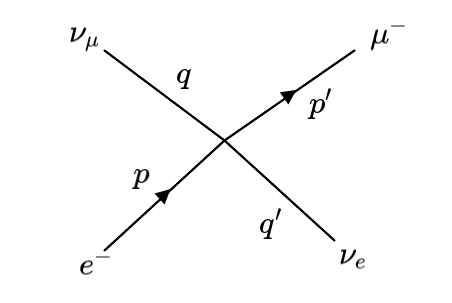
\includegraphics[width=\linewidth]{figs/diag_5.png}
\end{wrapfigure}
In the centre of mass frame, ignoring masses (i.e. at high energy)
\begin{equation}
\bigg(\frac{d\sigma}{d\Omega}\bigg)_{CoM} = \frac{1}{64\pi^2s}\frac{1}{2}\sum_{spins}|\mathcal{M}|^2 = \frac{1}{4\pi}G_F^2s.
\end{equation}
Using $s=4E^2$, $d\Omega = 2\pi\ d(\cos\theta)$,
\begin{equation}
\frac{d\sigma}{d\cos\theta} = \frac{2G_F^2}{\pi}E^2.
\end{equation}
Compare this with, for example, the equivalent result for $e^+e^- \to \mu^+\mu^-$:
\begin{equation}
\frac{d\sigma}{d\cos\theta} = \frac{\alpha^2}{4\pi E^2}(\cos^4\theta/2 + \sin^4\theta/2)
\end{equation}
QED cross-sections scale as $1/E^2$ as $E \to \infty$. But Fermi theory cross-sections rise as $E^2$ as $E \to \infty$. This is a disaster! $|\mathcal{M}|^2$ is a probability, so it must be bounded. It can be shown quite generally that any cross section can be decomposed using the partial wave approximation:
\begin{equation}
\sigma = \frac{4\pi}{E^2}\sum_j(2j+1)|f_j|^2
\end{equation}
where $|f_j|^2 \leq 1$, which follows from $S^\dagger S =1$. In other words, we define contributions $\sigma_j \leq \frac{4\pi}{E^2}(2j+1)$. We can see from dimensional arguments that the Lagrangian leads to unitarity violation. $[G_F]=-2$ and $[\sigma]=-2$ so because $E$ is the only scale then $\sigma \sim G_F^2E^2$. We can see that as $E \to \infty$ we will end up with infinite cross sections, violating unitarity. 
%
\subsection{Renormalisability}
%
We need to draw all the possible Feynman diagrams. Consider, for example, $\nu_e\bar{\nu}_\mu \to \nu_e\bar{\nu}_\mu$.
\begin{wrapfigure}{l}{0.4\linewidth}
  \centering
  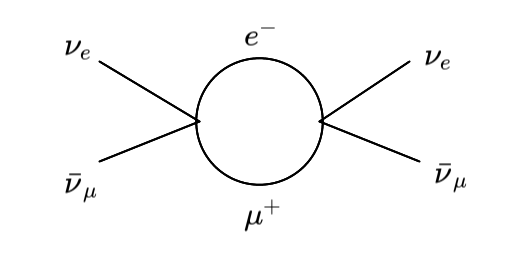
\includegraphics[width=\linewidth]{figs/diag_6.png}
\end{wrapfigure}
The vertex receives contributions from loop diagrams like the one shown here. But the loop gives contributions to the amplitude of the form
\begin{equation}
\sim \int d^4k \frac{\slashed{k}}{k^2}\frac{\slashed{k}}{k^2} \sim \int \frac{d^4k}{k^2}.
\end{equation}
In other words, the loop leads to quadratic divergences. But there is no $\bar{\nu}\nu\bar{\nu}\nu$ term in $\mathcal{L}$ to cancel this.
%
\subsection{Power counting}
%
Let's take QED as an example. Consider a graph with $L$ loops, $I_F$ fermion lines and $I_B$ photon lines. Considering the structure of contributions from Feynman rules, we can define the "superficial degree of divergence", $D$, to be
\begin{equation}
D = 4L - I_F - 2I_B.
\end{equation}
The logic here is that each loop contributes a $\int d^4k$ term, i.e. +4 powers of $k$. This gives the $4L$ term. Likewise, each fermion propagator contributes $\frac{\slashed{k}}{k^2}$, i.e. -1 powers of $k$, and each boson propagator contributes $\frac{1}{k^2}$, i.e. -2 powers of $k$. If $D \geq 0 $ then we would naively expect the graphs to lead to divergences. We can also impose the general result from graph theory that for $L$ loops, $I$ internal lines and $V$ vertices:
\begin{equation}
L = I - V + 1.
\end{equation}
The proof is by induction and left as an exercise. This means that
\begin{equation}
D = 2I_B + 3I_F - 4V + 4.
\end{equation}
Moreover, for QED we have the additional ammunition that there is only one type of vertex, joining two fermions and a photon. So, counting the ends of lines and labelling external lines $E$:
\begin{equation}
\begin{split}
&2I_B + E_B = V \\
&2I_F + E_F = 2V \\
\text{so } D &= V-E_B + \frac{3}{2}(2V-E_F) - 4V + 4 \\
&= 4 - E_B - \frac{3}{2}E_F
\end{split}
\end{equation}
i.e. $V$ cancels! $D$ is independent of $V$ and the only divergent graphs ($D \geq 0$) have corresponding counterterms which can regulate the divergences. The table enumerates the cases for QED where $D \geq 0$, explaining how each of these terms does in fact not lead to a divergence in this instance.
\begin{table}[h!]
\begin{tabular}{llll}
$E_B$ & $E_F$ & Diagram                                                 & Comments                                                                                              \\
\hline
2     & 0     & 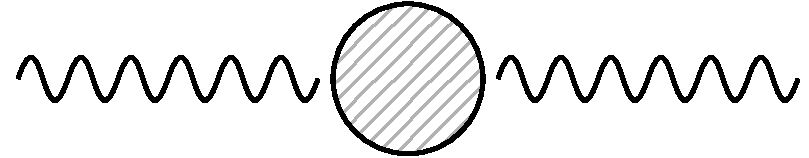
\includegraphics[scale=0.2]{figs/pc1.pdf} & $F_{\mu\nu}F^{\mu\nu}$, i.e. $Z_3$                                                                         \\
3     & 0     & 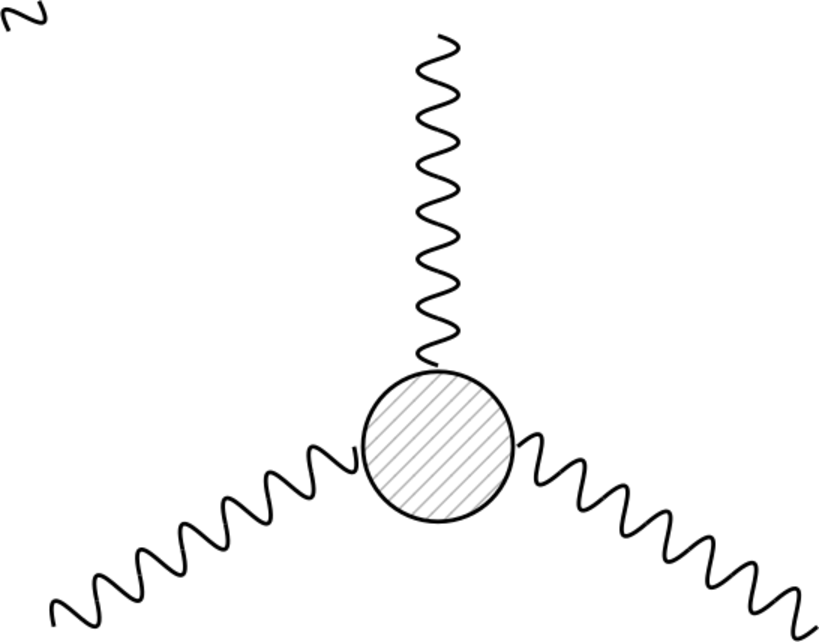
\includegraphics[scale=0.2]{figs/pc2.pdf}  & Photon is odd under $C$ so this gives 0 contribution                                                    \\ 
4     & 0     &  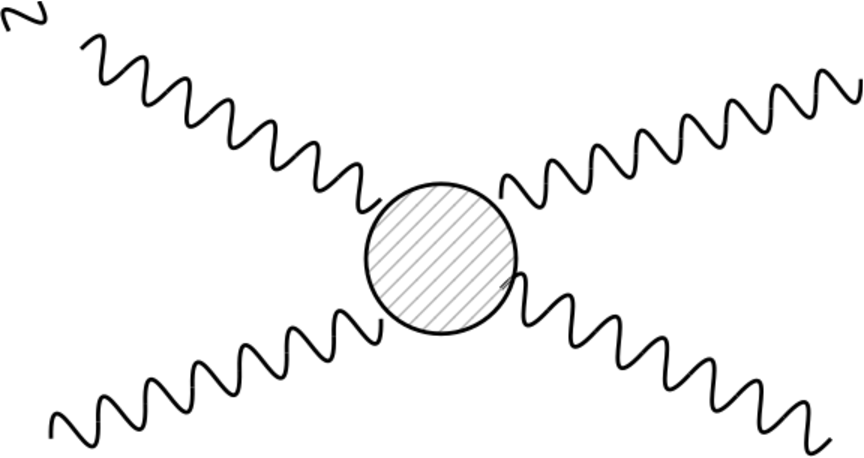
\includegraphics[scale=0.2]{figs/pc3.pdf}    & Actually finite (gauge invariance)                                                                    \\ 
0     & 2     & 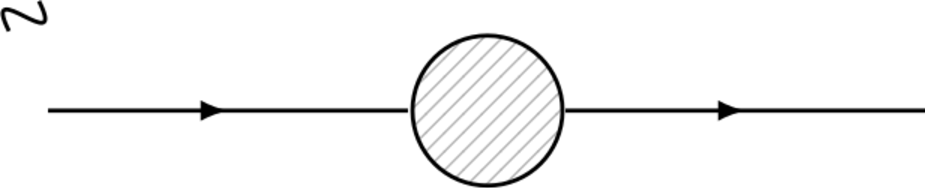
\includegraphics[scale=0.2]{figs/pc4.pdf}  & $\bar{\psi}\slashed{\partial}\psi + \bar{\psi}m\psi$, i.e. $Z_2$ and $Z_m$                            \\
2     & 1     & 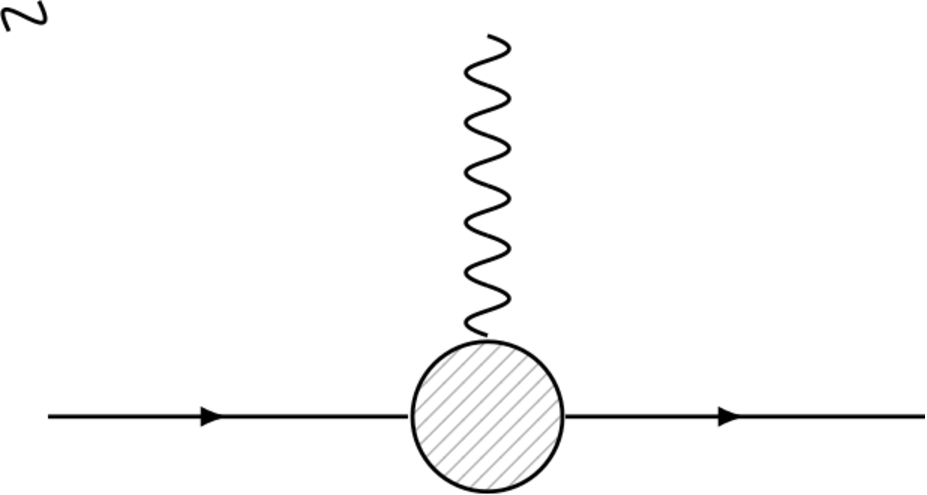
\includegraphics[scale=0.2]{figs/pc5.pdf} & 
$\bar{\psi}\slashed{A}\psi$, i.e. $Z_1$
\end{tabular}
\end{table}
In summary, QED is power-counting renormalisable. Note that if $E_F=4$ and $E_B=0$ then $D=-2$, i.e. the the four-fermion vertex is convergent.

Now let's move on from QED and consider $\mathcal{L}_{4F}$ instead. We can write the expression
\begin{equation}
2I_F + E_F = 4V
\end{equation}
so, if we only have fermions
\begin{equation}
\begin{split}
D &= \frac{3}{2}(4V-E_F) - 4V + 4 \\
&= 4 + 2V - \frac{3}{2} E_F.
\end{split}
\end{equation}
In other words,
\begin{enumerate}
\item every time we add a vertex, the graph becomes \textit{more} divergent
\item graphs with \textit{any} number of external fermions will diverge at a high enough order.
\end{enumerate}
For example, if $E_F = 6$, there are divergences for $V=3$. So $\mathcal{L}_{4F}$ is non-renormalisable. Adding bosons doesn't help the situation; we can trace the problem again to $[G_F]=-2$. 
\newline
\newline
\textbf{Theorem: } A theory is only power counting renormalisable if all the couplings have mass dimension $\geq 0$.
\newline
\textbf{Proof: } Consider a vertex $V_{bf}$ with $b$ boson lines, $f$ fermion lines and $p$ derivatives. The corresponding term in the Lagrangian is $g\phi^b\psi^f\partial^p$. The dimension of the coupling is
\begin{equation}
d_{bf}^p = 4 - b - \frac{3}{2}f - p
\end{equation}
because $[\mathcal{L}]=4$, $[\phi]=[A]=1$, $[\psi]=3/2$ and $[\partial]=1$. However,
\begin{equation}
\begin{split}
2I_B + E_B &= \sum bV_{bf}^p \\
2I_F + E_F &= \sum fV_{bf}^p \\
\text{so } D &= \sum bV_{bf}^p - E_B + \frac{3}{2}\big(\sum fV_{bf}^p - E_F\big) - 4 \sum V_{bf}^p + 4 + \sum p V_{bf}^p \\
&= \sum\big(b + \frac{3}{2}f + p - 4\big)V_{bf}^p - E_B - \frac{3}{2}E_F + 4 \\
&= -\sum d_{bf}^pV_{bf}^p - E_B - \frac{3}{2}E_F + 4.
\end{split}
\end{equation}
This means that for renormalisability we need $d_{bf}^p \geq 0$ so that $D$ increases as $V$ increases.
\newline
\textbf{Corollary: } For a theory with scalar, fermion and vector fields, the only vertices allowed in a renormalisable Lorentz invariant Lagrangian are:
\begin{table}[h!]
\begin{tabular}{ll}
 Pure scalar & $\psi^3$, $\psi^4$  \\
 Yang-Mills &  $\partial_\mu A_\nu A^\mu A^\nu$, $A_\mu A_\nu A^\mu A^\nu$ \\
 Gauge-scalar interactions & $\phi A_\mu A^\mu$, $\phi^2 A_\mu A^\mu$, $\phi \partial_\mu \phi A^\mu$ \\
 Yukawa &  $\phi \bar{\psi} \psi$ \\
 Gauge interactions & $\bar{\psi} \slashed{A} \psi$
\end{tabular}
\end{table}
\newline
\textbf{Proof: } $d^p_{bf} \geq 0$ only for the above. Note
\begin{itemize}
\item you need at least three fields
\item $A_\mu A^\mu A^\nu$, $\phi^2 \partial_\mu \phi$ and $\phi^2 A_\mu$ are not Lorentz invariant.
\end{itemize}
%
\subsection{Intermediate vector bosons}
%
Power counting renormalisability, chirality and Lorentz invariance suggest a vertex of the form $g\bar{\psi}_L\slashed{A}\psi_L$. Such a coupling is dimensionless so, following arguments from the previous section, unitarity is possible. This is the only possible coupling for left-handed fermions: the Yukawa coupling $\phi \bar{\psi}\psi = \phi(\bar{\psi}_L\psi_R + \bar{\psi}_R\psi_L)$ so is not a left-handed-only coupling. The charged currents are
\begin{equation}
\begin{split}
\frac{1}{2}J_\mu &= \bar{\nu}_e\gamma_\mu e_L + ... + \bar{u}_L \gamma_\mu d^\prime_L + ... \qquad \Delta Q = +1 \\
\frac{1}{2}J_\mu^\dagger &= \bar{e}_L \gamma_\mu \nu_e + ... + \bar{d}^\prime_L \gamma_\mu u_L + ... \qquad \Delta Q = -1
\end{split}
\end{equation}
so we need \textit{two} charged vector fields 
\begin{equation}
W_\pm^\mu = \frac{1}{\sqrt{2}} (W_1^\mu \pm i W_2^\mu)
\end{equation}
where $W_1^\mu$ and $W_2^\mu$ are real. Equivalently, we could define one complex field $W^\mu$, such that $W_+^\mu = W^\mu$ and $W_-^\mu = W^{\mu \dagger}$. The charged current Lagrangian can be written
\begin{equation}
\begin{split}
\mathcal{L}_{CC} &= \frac{g}{2\sqrt{2}}(J_\mu^\dagger W^\mu + W_\mu^\dagger J^\mu) \\
&= \frac{g}{\sqrt{2}}\bar{\nu}_e \slashed{W} e_L + \frac{g}{\sqrt{2}}\bar{e}_L \slashed{W}^\dagger \nu_e + ...
\end{split}
\end{equation}
where the factor of $2\sqrt{2}$ is conventional. $g$ is the (real) dimensionless coupling, and is the same for every term in $J_\mu$ (universality). 

$W_\mu$ is different from the $A_\mu$ in electromagnetism: 
\begin{itemize}
\item $W_\mu$ is charged, and thus complex
\item $W_\mu$ must be massive, because CC weak interactions are short range
\end{itemize}
In 1936 the Romanian physicist Alexandru Proca wrote down a Lagrangian to describe $W^\mu$, consisting of a kinetic term and a mass term:
\begin{equation}
\begin{split}
\mathcal{L}_W &= - \frac{1}{2}(\partial_\mu W_\nu - \partial_\nu W_\mu)^\dagger(\partial^\mu W^\nu - \partial^\nu W^\mu) + m_W^2 W_\mu^\dagger W^\mu \\
&\equiv -\frac{1}{2}W_{\mu \nu}^\dagger W^{\mu \nu} + m_W^2 W_\mu^\dagger W^\mu .
\end{split}
\end{equation}
So this gives an equation of motion
\begin{equation}
\begin{split}
&(\partial^2 + m_W^2) W^\mu - \partial^\mu \partial^\nu W_{\mu \nu} = 0 \\
&\implies \partial_\mu W^\mu =0 \text{ if } m_W \neq 0.
\end{split}
\end{equation}
We can look for plane wave solutions of the form $W^\mu = \epsilon^\mu e^{-i k \cdot x}$:
\begin{equation}
\begin{split}
(-k^2 + m_W^2)\epsilon^\mu + k^\mu k_\mu \epsilon^\nu &= 0 \\
\implies m_W^2 k_\mu \epsilon^\mu &= 0 
\end{split}
\end{equation}
where we have taken the physical solution in the last line. Since $W$ is massive it has three spin states: in the rest frame $k^\mu = (m_W, 0)$
\begin{equation}
\begin{split}
\epsilon_r^\parallel &= (0, \underline{\epsilon}_r) \qquad r=1,2,3 \\
\text{where } \qquad \underline{\epsilon}_1 &= (1,0,0) \\
\underline{\epsilon}_2 &= (0,1,0) \\
\underline{\epsilon}_3 &= (0,0,1). 
\end{split}
\end{equation}
$\underline{\epsilon}_1$ and $\underline{\epsilon}_2$ are the transverse components and can be combined to form $\underline{\epsilon}_\pm = 1/\sqrt{2}(1, \pm i, 0)$, and $\underline{\epsilon}_3$ is the longitudinal component. 

So if $k^\mu = (E, 0, 0, k)$, $\epsilon_3 = 1/m_W(k,0,0,E)$. N.B. for $E \gg m_W$, $\epsilon_3 \approx k^\mu/m_W + \mathcal{O}(m_W/E)$. Now let's evaluate the different polarisation sums: defining $\epsilon_0^\mu = k^\mu/m_W$ (so in the rest frame $\epsilon_0^\mu = (1, \underline{0})$ which is timelike, and therefore unphysical)
\begin{equation}
\begin{split}
&\sum_{r=0,1,2,3}\eta^{rr}\epsilon_r^\mu \epsilon_r^{\nu *} = - \eta^{\mu \nu} \qquad \text{completeness: cf RQFT} \\
\text{so } &\sum_{r=1,2,3}\epsilon^\mu_r \epsilon_r^{\nu *} = -\eta^{\mu \nu} + \epsilon_0^\mu \epsilon_0^\nu = -\eta^{\mu\nu} + \frac{k^\mu k^\nu}{m_W^2}
\end{split}
\end{equation}
The propagator is 
\begin{equation}
\Delta^{\mu\nu}_W = \frac{i(-\eta^{\mu \nu} + k^\mu k^\nu/m_W^2)}{k^2-m_W^2 + i\epsilon}
\end{equation}
because
\begin{equation}
\big((-k^2 + m_W^2)\eta_{\mu\nu} + k_\mu k_\nu)\Delta^{\nu \rho}_W = -i\delta_\mu^\rho
\end{equation}
(check this as an exercise).

The Feynman rule for the interaction is
\newline
\begin{wrapfigure}{l}{0.4\linewidth}
  \centering
  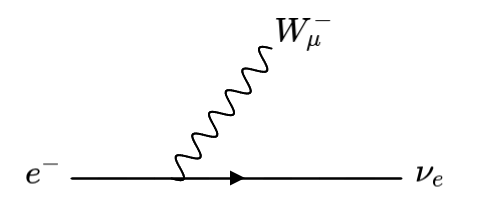
\includegraphics[width=\linewidth]{figs/17a.png}
\end{wrapfigure}
\begin{equation}
i\frac{g}{\sqrt{2}}\gamma_\mu\frac{1}{2}(1-\gamma^5)
\end{equation}
How does this theory work in practice? The following are some examples.
\newline
\newline
\subsubsection{$\mu^- \to e^-\bar{\nu}_e\nu_\mu$}
%\begin{wrapfigure}{r}{0.4\linewidth}
%  \centering
  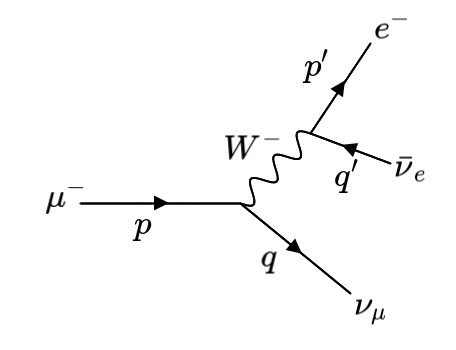
\includegraphics[width=0.4\linewidth]{figs/17b.png}
%\end{wrapfigure}
The momentum of $W^-$, $k=p-q=p^\prime + q^\prime$.
\begin{equation}
\begin{split}
\mathcal{M}& = \frac{(ig)^2}{8}\bar{u}(p^\prime)\gamma_mu(1-\gamma^5)v(q^\prime)\frac{(-\eta^{\mu \nu} + k^\mu k^\nu/m_W^2)}{k^2-m_W^2}\bar{u}(q)\gamma_\nu(1-\gamma^5)u(p) \\
\text{But } \qquad &\bar{u}(q)\slashed{k}(1-\gamma^5)u(p) = \bar{u}(q)(\slashed{p}-\slashed{q})(1-\gamma^5)u(p) = m_\mu \bar{u}(q)(1+\gamma^5)u(p) \\
&\bar{u}(p^\prime)\slashed{k}(1-\gamma^5)v(q^\prime) = \bar{u}(p^\prime)(\slashed{p}^\prime+\slashed{q}^\prime)(1-\gamma^5)v(q^\prime) = -m_e \bar{u}(p^\prime)(1+\gamma^5)v(q^\prime) 
\end{split}
\end{equation}
so the $k^\mu k^\nu/m_W^2$ term in the propagator tends to $m_e m_\mu/m_W^2 \sim 10^{-8}$ ($m_W=75$ GeV). Also $k^2 = m_\mu^2 - 2p \cdot q < m_\mu^2 \ll m_W^2$. If we ignore these terms, 
\begin{equation}
\frac{1}{2}\sum_{spins}|\mathcal{M}|^2 = \frac{2g^4}{m_W^4}(p \cdot q^\prime)(p^\prime \cdot q)
\end{equation}
i.e. this is the same as in 4-Fermi theory, provided that $G_F/\sqrt{2} = g^2/8m_W^2$. So the weak force is weak because $m_W$ is large ($\gg 1$ GeV). It is easy to see that the same arguments apply to \textit{all} weak decays in Chapter 1. 
%
\subsubsection{$\nu_\mu e^- \to \mu^- \nu_e$}
%
%\begin{wrapfigure}{r}{0.4\linewidth}
%  \centering
  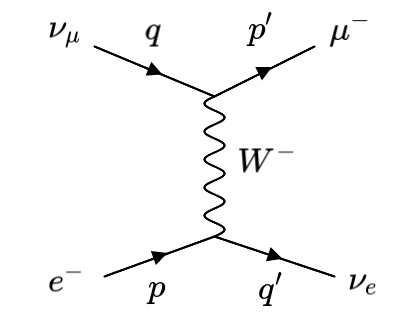
\includegraphics[width=0.3\linewidth]{figs/17c.png}
%\end{wrapfigure}
Here $k = p=q^\prime = p^\prime - q$ and
\begin{equation}
\mathcal{M} = \frac{(ig)^2}{8}\bar{u}(q^\prime)\gamma_\mu(1-\gamma^5)u(p)\frac{i(-\eta^{\mu\nu} + k^\mu k^\nu/m_W^2)}{k^2-m_W^2}\bar{u}(p^\prime)\gamma_\nu (1-\gamma^5)u(q).
\end{equation}
As before, $k^\mu k^\nu /m_W^2 \to m_e m_\mu /m_W^2$ so we can ignore these terms. But $k^2 = (p-q^\prime)^2 = t$ so
\begin{equation}
\frac{d\sigma}{d\Omega} = \frac{g^4}{128\pi^2}\frac{s}{(t-m_W^2)^2}
\end{equation}
where $s=4E^2$ and $t=-4E^2\sin^2\theta/2$. Integrating over $\phi$,
\begin{equation}
\begin{split}
\frac{d\sigma}{d\cos\theta} &= \frac{g^4E^2}{64\pi(E^2\sin^2\theta/2 + m_W^2/4)^2}
\\
&= \frac{g^4}{64\pi E^2}\csc^2 \frac{\theta}{2}\bigg( 1 + \mathcal{O}\big(\frac{m_W^2}{E^2}\big)\bigg).
\end{split}
\end{equation}
At very high energy, $E^2 \gg m_W^2$ so unitarity is restored. 
%
\subsubsection{$\nu \bar{\nu} \to W^+ W^-$}
%
Consider now the production of external $W^\pm$. In this case $q + q^\prime = k + k^\prime$. 
\newline
%
%\begin{wrapfigure}{r}{0.4\linewidth}
%  \centering
  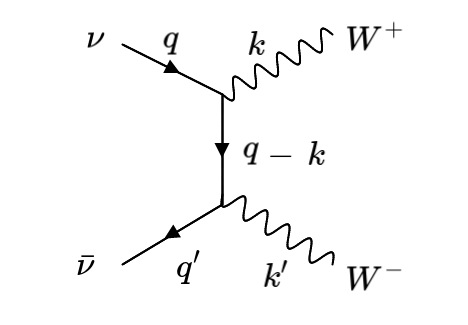
\includegraphics[width=0.4\linewidth]{figs/18a.png}
%\end{wrapfigure}
%
\begin{equation}
\mathcal{M} = \frac{(ig)^2}{8} \bar{v}(q^\prime) \gamma_\mu(1-\gamma^5)\frac{i(\slashed{q}-\slashed{k}+m_e)}{(q-k)^2 -m_e^2}\gamma_\nu(1-\gamma^5)u(q)\epsilon_r^\mu(k^\prime)^* \epsilon_r^\nu(k).
\end{equation}
We want the behaviour of the cross-section at very high energy, so we can ignore $m_e$. Also consider the $W$s to be longitudinally polarised, i.e. $\epsilon_3^\mu(k) \approx k^\mu/m_W + \mathcal{O}(m_W/E)$. So
\begin{equation}
\mathcal{M} = \frac{-ig^2}{4}\frac{1}{m_W^2(q-k)^2}\bar{v}(q^\prime)\slashed{k}^\prime(\slashed{q}-\slashed{k})\slashed{k}(1-\gamma^5)u(q)
\end{equation}
But $\slashed{q}u(q)=0$ so 
\begin{equation}
\begin{split}
\slashed{k}u(q) &= - (\slashed{q}-\slashed{k})u(q) \\
\text{similarly } \qquad \bar{v}(q^\prime)\slashed{k}^\prime &= \bar{v}(q^\prime)(\slashed{q}-\slashed{k})
\end{split}
\end{equation}
so if $p = q -k$, and recalling $\slashed{q}u(q)=0$)
\begin{equation}
\begin{split}
\mathcal{M} &= \frac{-ig^2}{4}\frac{1}{m_W^2p^2}\bar{v}(q^\prime)\slashed{p}\slashed{p}\slashed{p}(1-\gamma^5)u(q) \\
&= +\frac{ig^2}{4}\bar{v}(q^\prime)\slashed{k}(1-\gamma^5)u(q)
\end{split}
\end{equation}
and
\begin{equation}
\begin{split}
    \sum_{pol}|\mathcal{M}|^2 &= \frac{g^4}{16 m_W^4}\ tr\bigg(\slashed{q}^\prime \slashed{k}(1-\gamma^5)\slashed{q}\slashed{k}(1-\gamma^5)\bigg) \\
    & = \frac{g^4}{2m_W^4}(2q^\prime \cdot k q \cdot k - k^2 q \cdot q^\prime) \\
    & = \frac{g^4}{m_W^4} (q \cdot k q^\prime \cdot k - \frac{m_W^2}{2}q \cdot q^\prime).
\end{split}
\end{equation} 
Transforming to the Mandelstam variables, we can write
\begin{equation}
\begin{split}
s &= 2 q \cdot q^\prime, \\
t &= - 2 q \cdot k + m_W^2, \\
u &= - 2 q^\prime \cdot k + m_W^2,
\end{split}
\end{equation}
so
\begin{equation}
\begin{split}
    \sum_{pol}|\mathcal{M}|^2 &= \frac{g^4}{4m_W^4} \big(m_W^4 - (u + t + s)m_W^2 + ut\big)\\
    &= \frac{g^4}{4m_W^4} \big(m_W^4 - 2m_W^2 \times m_W^2 + ut\big)\\
 \text{so} \qquad   \frac{d\sigma}{d\Omega} &= \frac{g^4}{64\pi^2m_W^4}\frac{ut-m_W^4}{4s}.
\end{split}
\end{equation}
Considering the high energy limit, $E^2 \gg m_W^2$, so we can neglect the $m_W^4$ term, $s=4E^2$ and $ut = 4E^2\sin(\theta/2)\times 4E^2\cos(\theta/2) = 4E^4\sin^2\theta$. Integrating over $\phi$ in this limit,
\begin{equation}
\begin{split}
\frac{d\sigma}{d\cos\theta} &= \frac{g^4}{128\pi}\frac{E^2}{m_W^4}\sin^2\theta \\
\text{and} \qquad \qquad \sigma &= \frac{g^4}{128\pi}\frac{E^2}{m_W^4} \int_{-1}^1 d\cos\theta (1-\cos^2\theta) \\
&= \frac{g^4}{96\pi}\frac{E^2}{m_W^4}. 
\end{split}
\end{equation}
We can see that this violates unitarity! The cross section is unbounded as $E \to \infty$. It is clear that the $k_\mu k_\nu/m_W^2$ term in the $W$ propagator will spoil the power-counting renormalisability for graphs with internal $W$ lines coupled to internal fermions. 
%
\begin{wrapfigure}{l}{0.4\linewidth}
  \centering
  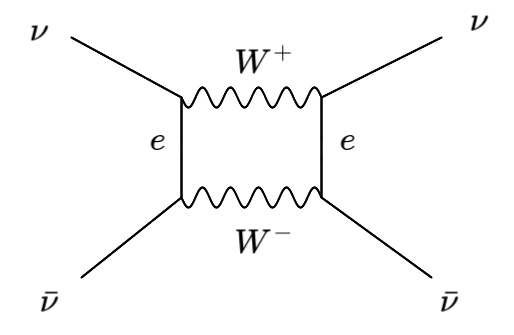
\includegraphics[width=\linewidth]{figs/18b.png}
\end{wrapfigure}
%
For example, this diagram has contributions
\begin{equation}
\sim \int d^4k \bigg(\frac{k^2/m_W^2}{k^2-m_W^2}\bigg)^2 \bigg(\frac{\slashed{k}}{k}\bigg)^2 \sim \int \frac{d^4k}{m_W^4k^2}.
\end{equation}
Unitarity and renormalisability of theories with vectors requires \textit{gauge invariance} under $W_\mu \to W_\mu + \partial_\mu \alpha \implies \epsilon_\mu \to \epsilon_\mu + \alpha k_\mu$. 
Remember that this problem doesn't arise in QED because for the comparitive process $\gamma e^- \to \gamma e^-$ we have two contributing diagrams:

%
%\begin{wrapfigure}{r}{0.7\linewidth}
%  \centering
  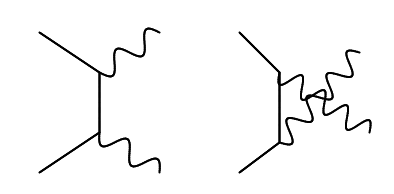
\includegraphics[width=\linewidth]{figs/18c.png}
%\end{wrapfigure}
%
\newline
whereas for EW, $W^+ \neq W^-$ so there is only one.

%
%\begin{wrapfigure}{r}{0.7\linewidth}
%  \centering
  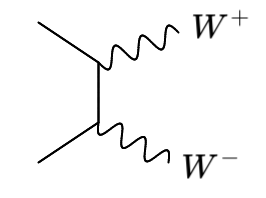
\includegraphics[width=0.4\linewidth]{figs/18d.png}
%\end{wrapfigure}
%
\newpage
%
\section{SU(2)$_L \otimes$U(1)$_V$ (Glashow, 1961)}
%
In the previous section we saw that in order to avoid unitarity violation we need to construct a gauge theory for the $W^\pm$ bosons. This must be:
\begin{itemize}
\item non-abelian, because abelian gauge bosons ($\gamma$) are neutral,
\item massive (how do we achieve this?).
\end{itemize}
The weak current $1/2 J_\mu = \bar{\nu}_e\gamma_\mu e_L + ...$ is built out of left-handed doublets:

\[ \psi_L \equiv \left( \begin{array}{cc}
\nu_e   \\
e   \end{array} \right)_L, \qquad
  \\ \left( \begin{array}{cc}
 \nu_\mu \\
\mu   \end{array} \right)_L, \qquad  \\ 
\left( \begin{array}{cc}
 \nu_\tau \\
\tau   \end{array} \right)_L \qquad\] 
and right-handed singlets 
$\psi_R \equiv e_R, \mu_R, \tau_R$. Notice that there is no $\nu_R$ because $\nu$ are massless. For now we are ignoring the quarks, and focussing on formulating a "theory of leptons". One obvious gauge group is SU(2) (or \textit{weak isospin}), with the $\psi_L$ and the $\psi_R$ in different representations because the weak interaction is \textit{chiral}. More explicitly,
\begin{equation}
\psi_L \to U \psi_L \qquad \text{and} \qquad \psi_R \to \psi_R, \qquad \text{where} \qquad U=\exp\bigg(\frac{i}{2}\underline{\alpha}\cdot\underline{\tau}\bigg) \in \text{SU(2)}.
\end{equation}
The dimension of SU(2) is 3, so there will be three gauge bosons. The hope is that these will correspond to $W^\pm, \gamma$. 

To see how the theory works in practice, consider explicitly writing

\[ \bar{\nu}_e\gamma_\mu e_L= \left( \begin{array}{c}
\nu_e \ e_L   \end{array} \right)
  \\ \left( \begin{array}{cc}
 0 \ 1 \\
1 \ 0   \end{array} \right)\gamma_\mu \\ 
\left( \begin{array}{cc}
 \nu_e \\
e_L   \end{array} \right). \qquad\] 
Now note that 
\[ \left( \begin{array}{cc}
 0 \ 1 \\
0 \ 0   \end{array} \right) = \frac{1}{2} 
\left( \begin{array}{cc}
 0 \ 1 \\
1 \ 0   \end{array} \right) + \frac{i}{2}
\left( \begin{array}{cc}
 0 \ -i \\
i \ \ 0   \end{array} \right) = \frac{1}{2}(\tau_1 + i\tau_2) \equiv T^+.
\qquad\] 
So
\begin{equation}
\begin{split}
\frac{1}{2}J_\mu &= \bar{\psi}_L T^+ \gamma_\mu \psi_L \\
\text{and} \qquad \frac{1}{2}J_\mu^\dagger &= \bar{\psi}_L T^- \gamma_\mu \psi_L,
\end{split}
\end{equation}
where 
\[ T^- = \frac{1}{2}(\tau_1 - i\tau_2) =
  \\ \left( \begin{array}{cc}
 0 \ 0 \\
1 \ 0   \end{array} \right). \qquad\]
Then, using the SU(2) relations
\begin{equation}
\begin{split}
&[T^+,T^-] = 2T_3, \\
&[T_3, T^\pm] = \pm T^\pm \\
\text{where} \qquad &T_3 = \frac{1}{2}\tau_3,
\end{split}
\end{equation}
we can compute the commutator
\begin{equation}
\begin{split}
[J_0^\dagger, J_0] &= \psi_L^\dagger[T^+,T^-]\psi_L \\
&=\psi_L^\dagger \ 2T^3 \psi_L \\
&= 2J_0^3.
\end{split}
\end{equation}
So we have three weak Noether currents:
\begin{equation}
\begin{split}
\underline{J}_\mu = (J_\mu^1, J_\mu^2, J_\mu^3) = \bar{\psi}_L \underline{T} \psi_L, \qquad \underline{T} = \frac{1}{2}\sigma, \\
\text{with} \qquad J_\mu^\pm = \frac{1}{2}(J_\mu^1 \pm iJ_\mu^2), \qquad J_\mu = J_\mu^+, \qquad J_mu^\dagger = J_\mu^-.
\end{split}
\end{equation}
Transforming in the adjoint representation of SU(2)$_L$ (i.e. the fundamental representation of SO(3)), we find
\begin{equation}
J_\mu^3 = \frac{1}{2}(\bar{\nu}_e \gamma_\mu \nu_e - \bar{e}_L \gamma_\mu e_L).
\end{equation}
This has $\Delta Q =0$ so it is a neutral current. However, it is \textit{not} the electromagnetic neutral current:
\begin{equation}
j_\mu = - \bar{e}\gamma_\mu e = - \bar{e}_L \gamma_\mu e_L - \bar{e}_R \gamma_\mu e_R,
\end{equation}
because this is vector-like and does not involve any neutrinos.
Considering the electric charge operator, $Q$:
\[ Q \psi_L = \left( \begin{array}{cc}
0 & 0  \\
0 & -1  \end{array} \right) \psi_L, \qquad
Q \psi_R = - \psi_R, \]
we can write $Q = T_3 + Y$, where $Y = (-1/2) \mathds{1}$ for left-handed leptons, and $Y = -1$ for right-handed leptons. Decomposed in the representation,
\[ Q \qquad = \qquad T_3 \qquad + \qquad Y: \]
\[\left( \begin{array}{cc}
0 & 0  \\
0 & -1  \end{array} \right)=
\left( \begin{array}{cc}
1/2 & 0  \\
0 & -1/2  \end{array} \right) +
\left( \begin{array}{cc}
-1/2 & 0  \\
0 & -1/2  \end{array} \right). \]
We call $Y$ the "weak hypercharge". It generates a U(1) symmetry of the form
\begin{equation}
\psi_L \to e^{-1/2 i \beta}\psi_L,  \qquad \psi_R \to e^{-i \beta}  \psi_R.
\end{equation}
Again, note the chiral structure.

Clearly the generators of SU(2)$_L$ and U(1)$_Y$ commute: the full symmetry group is SU(2)$_L \otimes$U(1)$_Y$, with elements $\exp{(i \underline{\alpha} \cdot \underline{T} + i \beta Y)}$. Overall, the Noether current is made up of a part belonging to SU(2)$_L$ and a part belonging to U(1)$_Y$, so we can write:
\begin{equation}
J_\mu^Y = j_\mu - J_\mu^3 = - \frac{1}{2}(\bar{\nu}_e \gamma_\mu \nu_e + \bar{e}_L \gamma_\mu e_L) - (\bar{e}_R \gamma_\mu e_R).
\end{equation}
From this starting point we want to build an SU(2)$_L \otimes$U(1)$_Y$ gauge theory. Considering the two individual groups,
\begin{equation}
\begin{split}
&\text{SU(2)}_L: \qquad \text{coupling \ } g, \qquad \text{gauge fields \ } \mathcal{W}_\mu \equiv \underline{W}_\mu \cdot \underline{T} \\
&\text{U(1)}_Y: \qquad \text{coupling \ } g^\prime, \qquad \text{gauge fields \ } B_\mu.
\end{split}
\end{equation}
The local symmetries are:
\begin{equation}
\begin{split}
&\mathcal{W}_\mu \to u \mathcal{W}_\mu u^\dagger + ig\ u \partial_\mu u^\dagger \\
&B_\mu \to B_\mu + i g^\prime \partial_\mu \beta,
\end{split}
\end{equation}
which translate to the covariant derivatives (using the hypercharge assignments):
\begin{equation}
\begin{split}
\mathcal{D}_\mu \psi_L &= (\partial_\mu - ig \mathcal{W}_\mu + i g^\prime \frac{1}{2} B_\mu) \psi_L, \\
\mathcal{D}_\mu \psi_R &= (\partial_\mu + i g^\prime B_\mu) \psi_R.
\end{split}
\end{equation}
Recalling that $\bar{\psi}\slashed{\partial}\psi = \psi_L \slashed{\partial} \psi_L + \psi_R \slashed{\partial} \psi_R$, we can write the Lagrangian explicitly as:
\begin{equation} 
\label{eqn:20a}
\begin{split}
\mathcal{L}_D &= \bar{\psi}_L i \mathcal{D} \psi_L +  \bar{\psi}_R i \mathcal{D} \psi_R \\
&= \bar{\psi} i \slashed{\partial} \psi + g \underline{W}^\mu \bar{\psi} \underline{T} \gamma_\mu \psi_L - g^\prime B^\mu \bigg( \frac{1}{2} \bar{\psi}_L \gamma_\mu \psi_L + \bar{\psi}_R \gamma_\mu \psi_R \bigg) \\
& = \bar{\psi} i \slashed{\partial} \psi + g \underline{W}^\mu \cdot \underline{J}_\mu + g^\prime B^\mu J_\mu^Y.
\end{split}
\end{equation}
Let's consider the charged current terms. We can write the complex field $W$ in terms of two real fields $W_1$ and $W_2$:
\begin{equation}
W^\mu = \frac{1}{\sqrt{2}} (W_1^\mu + i W_2^\mu), \qquad W^{\mu \dagger} = \frac{1}{\sqrt{2}} (W_1^\mu - i W_2^\mu).
\end{equation}
Now let's evaluate the terms in Eqn. \ref{eqn:20a} in turn, using $T^\pm = (T_1 \pm iT_2)$ and $W^\pm = 1/\sqrt{2}(W_1 \pm iW_2)$:
\begin{equation} \label{eqn:20b}
\begin{split}
\underline{T} \cdot \underline{W}^\mu &= \frac{1}{2} (T_1 + i T_2) (W_1^\mu + i W_2^\mu) + \frac{1}{2} (T_1 - i T_2)(W_1^\mu + i W_2^\mu) + T_3 W_3^\mu \\
&= \frac{1}{\sqrt{2}} (T^+ W^{\mu \dagger} + T^- W^\mu) + T_3 W_3^\mu,\\
g \underline{W}^\mu \cdot \underline{J}_\mu &= \frac{1}{2 \sqrt{2}} g(W^{\mu \dagger} J_\mu + J_\mu^\dagger W^\mu) + gJ_\mu^3 W_3^\mu.
\end{split}
\end{equation}
Looking at the last line of Eqn. \ref{eqn:20b}, the term in brackets is the charged current interaction, and the $gJ_\mu^3 W_3^\mu$ term is a new addition. 

Now let's consider the neutral current and electromagnetic terms. Clearly neither $W_\mu^3$ nor $B_\mu$ alone is the photon. Instead, the photon is produced through a mixture of the two. In general, we can write:
\[\left( \begin{array}{cc}
W^\mu_3 \\
B^\mu 
\end{array} \right) =
 \left( \begin{array}{cc}
\cos\theta_w & \sin\theta_w  \\
-\sin\theta_w & \cos\theta_w  \end{array} \right) 
\left( \begin{array}{cc}
Z^\mu \\
A^\mu 
\end{array} \right), \]
where $\theta_w$ is the weak mixing or "Weinberg" angle, to be determined. Substituting this explicitly into the expressions above leads to:
\begin{equation}
\begin{split}
gJ_\mu^3W_3^\mu + g^\prime(j_\mu - J_\mu^3)B^\mu &= \bigg((g\sin\theta_w - g^\prime \cos\theta_w)J_\mu^3 + g^\prime \cos\theta_wj_\mu\bigg)A^\mu \\
&+ \bigg((g\cos\theta_w + g^\prime \sin\theta_w)J_\mu^3 - g^\prime \sin\theta_w j_\mu\bigg)Z^\mu \\
&= ej_\mu A^\mu + \frac{g}{\cos\theta_w}\bigg(J_\mu^3 - \sin^2\theta_w j_\mu \bigg)Z^\mu,
\end{split}
\end{equation}
where we have inferred that $e = g^\prime \cos\theta_w = g \sin\theta_w$ is the electric charge. The first term is the QED part and the second term is the neutral current part. Note that $g, g^\prime$ are the same order as $e$: in fact, according to \textit{electroweak unification}, $1/e^2 = 1/g^2 + 1/g^{\prime 2}$, i.e. $e = g g^\prime/\sqrt{g^2 + g^{\prime 2}}$.

All in all the complete interaction is:
\begin{equation}
\begin{split}
ej_\mu A^\mu + &\frac{1}{2\sqrt{2}}g\big(W^{\mu \dagger}J_\mu + J_\mu^\dagger W^\mu \big) + \frac{g}{2 \cos\theta_w} J_\mu^{NC}Z^\mu, \\
\text{where } \qquad J_\mu^{NC} &= 2(J_\mu^3 - \sin^2\theta_w j_\mu) \\
&= 2\bigg( \frac{1}{2} (\bar{\nu}_L \gamma_\mu \nu_L - \bar{e}_L \gamma_\mu e_L) + \sin^2\theta_w \bar{e} \gamma_\mu e \bigg) \\
&= \bar{\nu}_L \gamma_\mu \nu_L + \bar{e} \gamma_\mu \big( (2\sin^2\theta_w - \frac{1}{2}) + \frac{1}{2} \gamma^5 \big) e \\
&\equiv \bar{\nu}_L \gamma_\mu \nu_L + \bar{e} \gamma_\mu \big(c_V + c_A \gamma^5 \big)e.
\end{split}
\end{equation}
So the neutral current is not pure V-A, but instead a mixture of left and right:
\begin{equation}
\begin{split}
&c_V- c_A\gamma^5 = c_L P_L + c_R P_R \\
\text{where} \qquad &c_L = c_V + c_A = 2 \sin^2\theta_w -1, \qquad c_R = c_V-c_A = 2 \sin^2\theta_w.
\end{split}
\end{equation}
The Feynman rule corresponding to the neutral current vertex is
%
\newline
%\begin{wrapfigure}{l}{\linewidth}
  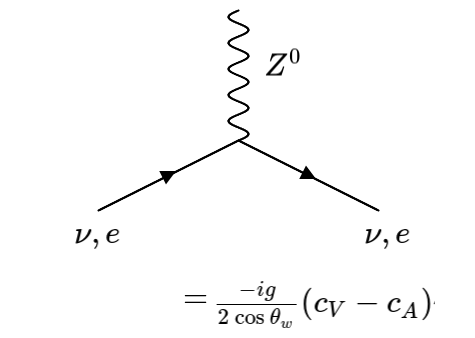
\includegraphics[width=0.4\linewidth]{figs/21a.png}
%\end{wrapfigure}
\newline
where for neutrinos $c_V = c_A = 1/2$ and for electrons $c_V = -1/2 + 2\sin\theta_w$ and $c_A = -1/2$. We can also write down gauge invariant vector boson kinetic terms
\begin{equation} \label{eqn:22a}
\begin{split}
\mathcal{L}_{YM} &= - \frac{1}{2} tr \mathcal{W}^{\mu \nu} \mathcal{W}_{\mu \nu} - \frac{1}{4} B^{\mu \nu} B_{\mu \nu}, \\
\text{where} \qquad \mathcal{W}_{\mu \nu} &= \partial_\mu \mathcal{W}_\nu - \partial_\nu \mathcal{W}_\mu -ig[\mathcal{W}_\mu, \mathcal{W}_\nu] \qquad \text{SU(2)}_L \text{: nonabelian}, \\
B_{\mu \nu} &= \partial_\mu B_\nu - \partial_\nu B_\mu \qquad \qquad \qquad \qquad \qquad \text{U(1)}_Y \text{: abelian}.
\end{split}
\end{equation}
Now expand in terms of the generators:
\begin{equation}
\begin{split}
\mathcal{W}_\mu &= \frac{1}{\sqrt{2}}(W_\mu^\dagger T^+ + W_\mu T^-) + W_\mu^3 T_3, \\
\mathcal{W}_{\mu \nu} &= \frac{1}{\sqrt{2}}(W_{\mu \nu}^\dagger T^+ + W_{\mu \nu} T^- ) + W_{\mu \nu} ^3 T_3
\end{split}
\end{equation}
and substitute into Eqn. \ref{eqn:22a}. Applying the commutation relations $[T^+, T^-] = 2 T_3$ and $[T_3, T^\pm] = \pm T^\pm$, and then equating terms proportional to each of the generators yields:
\begin{equation}
\begin{split}
W_{\mu \nu} &= \partial_\mu W_\nu - \partial_\nu W_\mu -ig(W_\mu^3 W_\nu - W_\nu^3 W_\mu), \\
W_{\mu \nu}^3 &= \partial_\mu W_\nu^3 - \partial_\nu W_\mu^3 - ig(W_\mu^\dagger W_\nu - W_\nu^\dagger W_\mu).
\end{split}
\end{equation}
Now using the fact that $tr \ T_1^2 + T_2^2 = tr\ T_-T_+ = 1$ and $tr \ T_3^2 = 1/2$, we can rephrase the Lagrangian as:
\begin{equation}
\begin{split}
\mathcal{L}_{YM} = &-\frac{1}{2} W_{\mu \nu}^\dagger W^{\mu \nu} = \frac{1}{4} W_{\mu \nu}^3 W^{\mu \nu}_3 - \frac{1}{4}B_{\mu \nu} B^{\mu \nu} \\
= &- \frac{1}{2}(\partial_\mu W_\nu^\dagger - \partial_\nu W_\mu^\dagger)(\partial^\mu W^\nu - \partial^\nu W^\mu)\\ &- \frac{1}{4}(\partial_\mu Z_\nu - \partial_\nu Z_\mu)^2 - \frac{1}{4}(\partial_\mu A_\nu - \partial_\nu A_\mu)^2 + \mathcal{L}_{YM}^3 + \mathcal{L}_{YM}^4,
\end{split}
\end{equation}
where $\mathcal{L}_{YM}^3$ and $\mathcal{L}_{YM}^4$ are the interaction terms:
\begin{equation}
\begin{split}
\mathcal{L}_{YM}^3 = &ig \bigg( (\partial_\mu W_\nu^\dagger - \partial_\nu W_\mu^\dagger) W_3^\mu W^\nu - W_3^\mu W^{\nu \dagger}(\partial_\mu W_\nu - \partial_\nu W_\mu) \\ &+ (\partial_\mu W_\nu^3 - \partial_\nu W_\mu^3) W^{\mu \dagger} W^\nu \bigg), \\
\mathcal{L}_{YM}^4 = &g^2 \bigg( \frac{1}{4}(W_\mu^\dagger W_\nu - W_\nu^\dagger W_\mu)^2 - (W_\mu^3 W_\nu^\dagger - W\nu^3 W_\mu^\dagger) W_3^\mu W^\nu \bigg).
\end{split}
\end{equation}
The weak mixing matrix is orthogonal, which means $W_3^2 + B^2 = Z^2 + A^2$ so we end up with the usual kinetic terms for $W, Z, \gamma$. Finally, using the relations $W_\mu^3 = \cos\theta_wZ^\mu + \sin\theta_w A^\mu$ and $g=e/\sin\theta_w$, we have the following Feynman rules:
\newline
\begin{figure}[!h]
  \centering
  \subfloat[triple vertex]{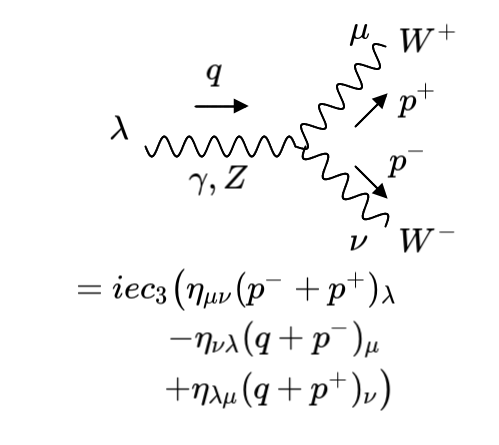
\includegraphics[width=0.5\textwidth]{figs/22a.png}}
  \hfill
  \subfloat[quartic vertex]{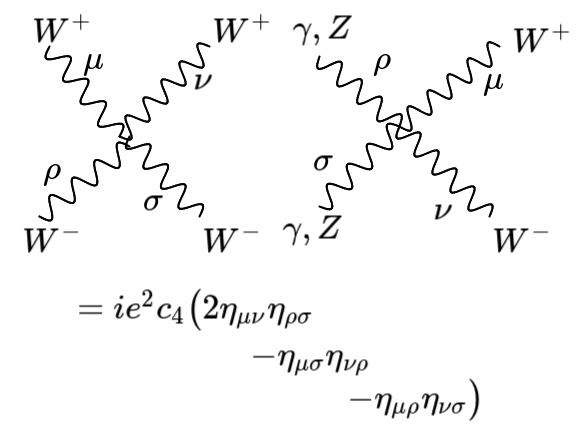
\includegraphics[width=0.5\textwidth]{figs/22b.png}}
\end{figure}
\newline
where 
\begin{equation}
c_3 =
\begin{cases}
1 \qquad \qquad \text{for } \gamma\\
\cot\theta_w \qquad \text{for } Z,
\end{cases}
\end{equation}
and

\begin{equation}
c_4 =
\begin{cases}
\csc^2\theta_w \qquad \text{for } WWWW\\
-1 \qquad \qquad \text{for } WW\gamma \gamma \\
-\cot\theta_w \qquad \text{for } WWZ \gamma \\
-\cot^2\theta_w \qquad \text{for } WWZZ.
\end{cases}
\end{equation}
Note that the photon couples to the electric charge of the $W^\pm$: there is no dependence on $\theta_w$. There are no couplings which only involve $\gamma$ and $Z^0$, as the $Z^0$ is neutral and $\gamma$ only couples to electrically charged particles. It is easy to show that $\mathcal{L}_{YM}$ is gauge invariant under U(1)$_Q$ if the $Z$ is ignored (Exercise). 
%
\subsection{The Z mass}
%
Clearly the $Z^0$ must be heavy, like $W^\pm$, otherwise the neutral current interactions would be long-range. We can introduce a mass term by hand, just as we did for the $W^\pm$, ensuring it is consistent with \textit{global} SU(2)$_L \otimes$U(1)$_Y$ symmetry. Remember that such a term will always break gauge invariance. The most general mass term is
\begin{equation}
\mathcal{L}_M  = m_W^2 W_\mu^\dagger W^\mu + \frac{1}{2} W_\mu^3 W_3^\mu + \frac{1}{2}m_B^2 B_\mu B^\mu.
\end{equation}
However, this can't be correct: the mass eigenstates are $Z_\mu$ and $A_\mu$, and the photon ($A_\mu$) is massless. We saw above that $W_\mu^3$ and $B_\mu$ mix. We can assume this mixing is in the mass matrix, which will mean it has no effect at high energy (where the masses are negligible). This is known as \textit{soft breaking}. In this case,
\begin{equation}
\mathcal{L}_{gauge}^{mass} \to \mathcal{L}_{gauge}^{mass} - m_X^2W_\mu^3 B^\mu,
\end{equation}
and we can write the mass matrix for $W_\mu^3$ and $B_\mu$ as:
\[ \left( \begin{array}{cc}
m_W^2 & -m_X^2  \\
-m_X^2 & m_B^2  \end{array} \right).  \]
We know because the photon is massless that this must have a zero eigenvalue. This fixes $m_X^2 = m_W m_B$. Moreover, we know that the corresponding zero eigenvector is
$A_\mu = \sin\theta_w W_\mu^3 + \cos\theta_w B_\mu$, so 
\[ \left( \begin{array}{cc}
m_W^2 & -m_Wm_B  \\
-m_Wm_B & m_B^2  \end{array} \right)
\left( \begin{array}{cc}
\sin\theta_w \\
\cos\theta_w \end{array} \right) = 0 \\
\implies m_B\cos\theta_w = m_W\sin\theta_w. \]
The other eigenvalue is 
\begin{equation}
\begin{split}
m_Z^2 &= m_W^2 + m_B^2 \\
&= m_W^2(1+ \tan^2\theta_w) \\
&= \frac{m_W^2}{\cos\theta_w} > m_W^2.
\end{split}
\end{equation}
Note that the fermion mass terms $\mathcal{L}_m = m(\bar{\psi}_L\psi_R + \bar{\psi}_R \psi_L)$ also break SU(2)$_L \otimes$U(1)$_Y$, and mix the SU(2) doublets (left-handed fermions) with the U(1) singlets (right-handed fermions). 
%
\subsubsection{Summary}
%
\begin{itemize}
\item SU(2)$_L \otimes$U(1)$_Y$ symmetry remains at high energy,
\item $g = e/\sin\theta_w$: QED and electroweak are unified,
\item we predict a new \textit{neutral current} weak interaction with mass $m_Z = m_W/\cos\theta_w$,
\item mass terms for both vector bosons and fermions break the SU(2)$_L \otimes$U(1)$_Y$ symmetry by mixing.
\end{itemize}
%
\subsection{Neutral Currents}
%
Neutral currents are \textit{chiral}: they involve both left-handed and right-handed components but not equally, and they can involve neutrinos. However, they do \textit{not} change flavour, e.g. they don't change electrons into neutrinos. We say that there are no "flavour changing neutral currents" (FCNCs). 

The $Z_0$ is heavy (in fact it is heavier than the $W^\pm$), and has the propagator
\begin{equation}
\Delta_Z^{\mu \nu} = \frac{i(-\eta^{\mu \nu} + k^\mu k^\nu/m_Z^2)}{k^2 - m_Z^2 + i \epsilon},
\end{equation}
and polarisation vectors $\epsilon_\mu^r(k)$, $r=1,2,3$ as for the $W$. At low energies $k^2 \ll m_Z^2$ and you end up with a new effective four-fermion interaction:
\newline
%\begin{wrapfigure}{l}{\linewidth}
  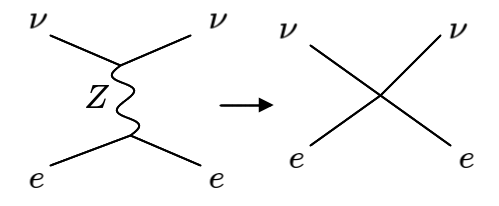
\includegraphics[width=0.6\linewidth]{figs/24a.png}
%\end{wrapfigure}
\newline
with an effective Lagrangian
\begin{equation}
\mathcal{L}_{4F} \to \frac{-g^2}{8m_W^2}(J_\mu^\dagger J^\mu + \rho J_\mu^{NC}J^\mu_{NC}),
\end{equation}
where $\rho = m_W^2/\cos^2\theta_w m_Z^2 =1$ is the Veltman parameter. Neutral current interactions are very difficult to see at low energy because of the  presence of the neutral electromagnetic current $\gamma$. Neutral current interactions were first observed at Garganelle (CERN) in 1973, in neutrino scattering off a nucleus: $\nu_\mu N \to \nu_\mu N$. These experiments are very difficult as the neutrino beam comes from pion decays at a rate of just 3 events in 2 years!
%
\subsubsection{Example: $\nu_\mu e^- \to \nu_\mu e^-$}
%
Let's first consider the process at low energy, as an effective theory.
\newline
%\begin{wrapfigure}{l}{\linewidth}
  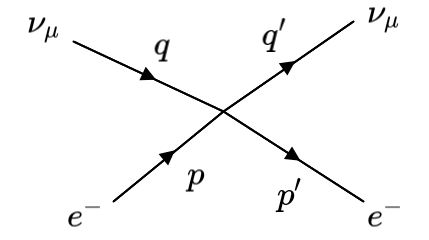
\includegraphics[width=0.4\linewidth]{figs/24b.png}
%\end{wrapfigure}
\newline
\begin{equation}
\mathcal{M} = \frac{-iG_F}{\sqrt{2}} \rho \bar{u}(p^\prime) \gamma_\mu(c_V - c_A \gamma^5) u(p) \bar{u}(q^\prime) \gamma^\mu (1-\gamma^5) u(q),
\end{equation}
so averaging over initial spins and summing over final spins gives
\begin{equation}
\begin{split}
\frac{1}{2}\sum_{spins}|\mathcal{M}|^2 &= \frac{G_F^2\rho^2}{2}\ tr \bigg(\slashed{p}^\prime \gamma_\mu(c_V-c_A\gamma^5)\slashed{p}\gamma_\nu(c_V-c_A \gamma^5)\bigg)\ tr \bigg(\slashed{q}^\prime \gamma^\mu(1-\gamma^5)\slashed{q}\gamma^\nu(1-\gamma^5)\bigg) \\
&= 32G_F^2 \rho^2 \bigg( (c_V^2+c_A^2)(p_\mu p^\prime_\nu + p^\prime_\mu p_\nu - \eta_{\mu \nu} p\cdot p^\prime) - 2ic_Vc_A \epsilon_{\mu \nu \alpha \beta}p^\alpha p^{\prime \beta}\bigg) \\
&\times \bigg(q^\mu q^{\prime \nu} + q^{\prime \mu} q^\nu -\eta^{\mu \nu} q \cdot q^\prime - i\epsilon^{\mu \nu \rho \sigma}q_\sigma q^\prime_\rho \bigg) \\
&= 64G_F^2 \rho^2 \bigg( (c_V^2+c_A^2)(p \cdot q p^\prime \cdot q^\prime + p\cdot q^\prime p^\prime \cdot q) + 2c_Vc_A(p \cdot q p^\prime \cdot q^\prime - p\cdot q^\prime p^\prime \cdot q) \bigg) \\
&= 64G_F^2 \rho^2 \bigg((c_V+c_A)^2 p \cdot q p^\prime \cdot q^\prime + (c_V-c_A)^2 p \cdot q^\prime p^\prime \cdot q \bigg) \\
&= 16 G_F^2\rho^2(c_L^2s^2 + c_R^2u^2)
\end{split}
\end{equation}
where we have used $c_L = c_V + c_A$ and $c_R = c_V-c_A$, and the Mandelstam variables $s=2 p \cdot q = 4E^2$ and $u=-2p \cdot q^\prime = -2E^2(1+ \cos\theta)$. We can now calculate the total cross section by integrating first over $\phi$ and then over $\theta$:
\begin{equation}
\begin{split}
\frac{d\sigma}{d\cos\theta} &= \frac{G_F^2 \rho^2}{2 \pi} E^2 \big(c_L^2 + c_R^2\frac{1}{2}(1 + \cos^2\theta)\big) \\
\implies \sigma(\nu_\mu e) &= \frac{G_F^2 \rho^2 E^2}{\pi} \big(c_L^2 + \frac{1}{3}c_R^2\big) \\
&= \frac{4G_F^2 \rho^2E^2}{3 \pi}\big(c_V^2 + c_A^2 + c_V c_A\big).
\end{split}
\end{equation}
You can infer $\sigma(\bar{\nu}_\mu e)$ from crossing symmetry $q \leftrightarrow q^\prime$, or $c_A \leftrightarrow -c_A$, $c_L \leftrightarrow c_R$. So the ratio of these two cross sections is
\begin{equation}
\frac{\sigma(\bar{\nu}_\mu e)}{\sigma(\nu_\mu e)} = \frac{c_V^2 + c_A^2 - c_Vc_A}{c_V^2 + c_A^2 + c_V c_A},
\end{equation}
where in this instance $c_V = 2 \sin^2\theta_w -1/2$ and $c_A = -1/2$. From this we can deduce that $\sin^2\theta_w \approx 0.23$. 

For the high-energy cross section we need to take account of the $Z^0$ propagator.
\begin{wrapfigure}{l}{0.3\linewidth}
  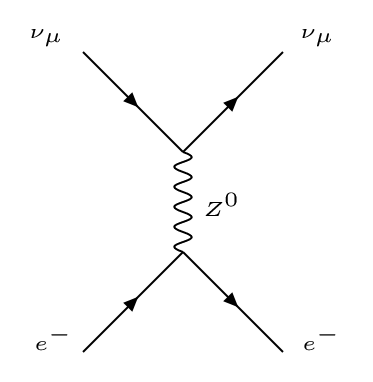
\includegraphics[width=\linewidth]{figs/25a.png}
\end{wrapfigure}
This corresponds to replacing 
\begin{equation}
-i\eta^{\mu\nu} \to i(-\eta^{\mu\nu} + k^\mu k^\nu/m_Z^2)/k^2-m_Z^2.
\end{equation} 
But remember that 
\begin{equation}
\bar{u}(q^\prime)\slashed{k}(1-\gamma^5)u(q) = \bar{u}(q^\prime)(\slashed{q}-\slashed{q}^\prime)(1-\gamma^5)u(q)=0,
\end{equation}
so in fact we can ignore the $k^\mu k^\nu/m_Z^2$ term, and only need to address the change in the denominator. 
\begin{equation}
k^2 = t = -2E^2(1-\cos\theta),
\end{equation}
so the total differential cross section becomes
\begin{equation}
\frac{d\sigma}{d\cos\theta} = \frac{e^4}{\pi\sin^2\theta_w}\frac{E^2}{(m_Z^2 + 2E^2(1-\cos\theta))^2}\big(c_L^2 + c_A^2 \frac{1}{2}(1+\cos\theta)^2\big).
\end{equation}
You can see that in this case unitarity is retained in the limit $E^2 \gg m_Z^2$.
%
\subsubsection{Example: $e^+ e^- \to \mu^+ \mu^-$}
%
\begin{figure}[!h]
  \centering
  \subfloat[QED]{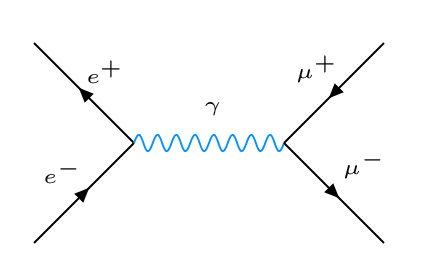
\includegraphics[width=0.5\textwidth]{figs/25b.png}}
  \hfill
  \subfloat[NC]{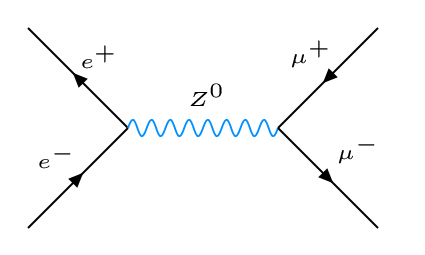
\includegraphics[width=0.5\textwidth]{figs/25c.png}}
\end{figure}
This is a standard process occurring at $e^+ e^-$ colliders, and is a very sensitive test of NC electroweak theory. See the examples sheet.
%
\subsubsection{Example: $\nu \bar{\nu} \to W^+W^-$ again}
%
We saw earlier that the diagram in the $t$-channel violates unitarity. We now have a new graph in the $s$-channel, representing the contribution from the $Z^0$.
\begin{figure}[!h]
  \centering
  \subfloat[$t$-channel]{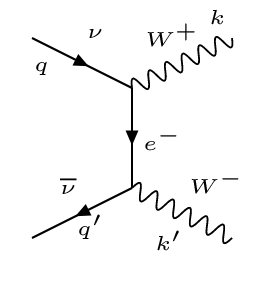
\includegraphics[width=0.3\textwidth]{figs/26a.png}}
  \hfill
  \subfloat[$s$-channel]{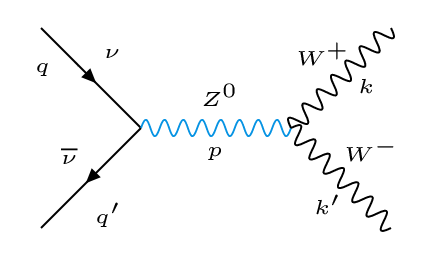
\includegraphics[width=0.5\textwidth]{figs/26b.png}}
\end{figure}
Does the addition of this diagram restore unitarity? We need to compute the total amplitude $\mathcal{M} = \mathcal{M}_t + \mathcal{M}_s$. We already worked out that
\begin{equation}
\mathcal{M}_t = \frac{+ig^2}{4m_W^2}\bar{v}(q^\prime)\slashed{k}(1-\gamma^5)u(q),
\end{equation}
and we can use the Feynman rules in the $s$-channel to write
\begin{equation}
\begin{split}
\mathcal{M}_s = \frac{+ig}{4\cos\theta_w}\bar{v}(q^\prime)\gamma_\mu(1-\gamma^5)u(q)i\frac{-\eta^{\mu \nu}+p^\mu p^\nu/m_Z^2}{p^2-m_Z^2}(ig\cos\theta_w) \\
\times \bigg(\eta_{\alpha \beta}(k^\prime - k)_\nu - \eta_{\beta \nu} (p + k^\prime)_\alpha + \eta_{\alpha \nu}(p+k)_\beta \bigg)\frac{k^\alpha}{m_W}\frac{k^{\prime \beta}}{m_W},
\end{split}
\end{equation}
where we have used the high energy limits to simplify the external $W$ lines, and that, for $\nu$, $c_V = c_A = 1/2$.

Let's look first at the $p^\mu p ^\nu$ term, using $p=q+q^\prime = k + k^\prime$ and matching up all the indices:
\begin{equation}
\begin{split}
&(k \cdot k^\prime) p \cdot(k^\prime - k) - (p \cdot k^\prime)(p+k^\prime)\cdot k + (p \cdot k)(p+k) \cdot k^\prime \\
=\ &(k \cdot k^\prime)p\cdot(k^\prime-k) + k\cdot k^\prime (p\cdot k - p \cdot k^\prime) \\
=\ &0.
\end{split}
\end{equation}
So we are just left with the $-\eta^{\mu \nu}$ term:
\begin{equation}
\begin{split}
&- \big( (k \cdot k^\prime)(k^\prime_\mu - k_\mu) - k_\mu^\prime (p+k^\prime)\cdot k + k_\mu (p+k)\cdot k^\prime \big) \\
=\ &p \cdot k k^\prime_\mu - p \cdot k^\prime k_\mu,
\end{split}
\end{equation}
but 
\begin{equation}
\bar{v}(q^\prime)\slashed{k}^\prime(1-\gamma^5)u(q) = -\bar{v}(g^\prime)\slashed{k}(1-\gamma^5)u(q),
\end{equation}
so altogether
\begin{equation}
\mathcal{M}_s = -\frac{ig}{4m_W^2}v(q^\prime)\slashed{k}(1-\gamma^5)u(q) \frac{p \cdot (k + k^\prime)}{p^2-m_Z^2},
\end{equation}
and
\begin{equation}
\begin{split}
\mathcal{M}_t + \mathcal{M}_s = \frac{ig^2}{4m_W^2}\bar{v}(q^\prime)\slashed{k}(1-\gamma^5)u(q)\bigg(1-\frac{p^2}{p^2-m_Z^2}\bigg).
\end{split}
\end{equation}
The bracketed term on the right can be re-expressed as $-m_Z^2/(p^2-m_Z^2) = -m_Z^2/(s-m_Z^2)$, so 
\begin{equation}
\mathcal{M}_t + \mathcal{M}_s = -{ig^2}{4\cos^2\theta_w}\frac{1}{s-m_Z}^2\bar{v}(q^\prime)\slashed{k}(-\gamma^5)u(q).
\end{equation}
Squaring as before, we arrive at
\begin{equation}
\frac{d\sigma}{d\Omega} = \frac{g^4}{64\pi^2\cos\theta_w}\frac{ut-m_W^4}{s(s-m_Z^2)^2},
\end{equation}
so for $E^2 \gg m_W^2$
\begin{equation}
\frac{d\sigma}{d\cos\theta} = \frac{1}{16E^2}\frac{g^4\sin^2\theta}{128\pi\cos^4\theta_w}.
\end{equation}
Thankfully, unitarity is restored! (N.B. Remember that we took the high energy limit in the $\epsilon_\mu$ terms for external $W$ bosons. The sub-leading terms give an additional factor of $\cos^22\theta_w$.) 

However, there are still processes which violate unitarity, such as $W^+W^- \to W^+W^-$. There is also no improvement in the issue of power-counting renormalisability. 
%
\subsection{Hadronic Neutral Current}
%
Remember the expression for hadronic charged current:
\begin{equation}
\frac{1}{2}J_\mu^h = \bar{u}_L \gamma_\mu d^\prime_L + ...,
\end{equation}
so we have left-handed doublets
\[ q_L = \left( \begin{array}{cc}
u   \\
d^\prime   \end{array} \right)_L, \qquad
  \\ \left( \begin{array}{cc}
 c \\
s^\prime   \end{array} \right)_L, \qquad  \\ 
\left( \begin{array}{cc}
 t \\
b^\prime   \end{array} \right)_L; \qquad\] 
and right-handed singlets $q_R = u_R, d_R, c_R, s_R, t_R, b_R$.  So
\begin{equation}
\underline{J}^h_\mu = \bar{q}_L \underline{T} \gamma_\mu q_L,
\end{equation}
i.e.
\begin{equation}
J_\mu^{3\ h} = \frac{1}{2}\bar{u}_L \gamma_\mu u_L - \frac{1}{2} \bar{d}_L^\prime \gamma_\mu d_L^\prime + ...,
\end{equation}
while the electromagnetic current is
\begin{equation}
j_\mu^h = \frac{2}{3} \bar{u} \gamma_\mu u - \frac{1}{3} \bar{d}^\prime \gamma_\mu d^\prime + ...,
\end{equation}
corresponding to 
\[ Q = \left( \begin{array}{cc}
2/3 & 0   \\
0 & -1/3   \end{array} \right). \qquad \]
Using this to evaluate the weak hypercharge,
\begin{equation}
Y = Q - T_3 =
\begin{cases}
+\frac{1}{6}\mathds{1} \qquad \qquad \text{for LH doublets} \\
+\frac{2}{3} \qquad \qquad \text{  for } u_R, c_R, t_R \\
-\frac{1}{3} \qquad \qquad \text{  for } d_R, s_R, b_R. 
\end{cases}
\end{equation}
The netural-current can then be expressed:
\begin{equation}
\begin{split}
J_\mu^{NC\ h} &= 2 (J_\mu^{3\ h} - \sin^2\theta_w j_\mu^h) \\
&= 2 \bar{q} \gamma_\mu \bigg(\frac{1}{2} T_3 (1-\gamma^5) - Q \sin^2\theta_w \bigg) q \\
&= \bar{u} \gamma_\mu \bigg( -\frac{4}{3}\sin^2\theta_w + \frac{1}{2}(1-\gamma^5)\bigg) u + \bar{d}^\prime \gamma_\mu \bigg(\frac{2}{3} \sin^2\theta_w - \frac{1}{2}(1 - \gamma^5) \bigg) d^\prime + ...
\end{split}
\end{equation}
This corresponds to the Feynman rule
\newline
  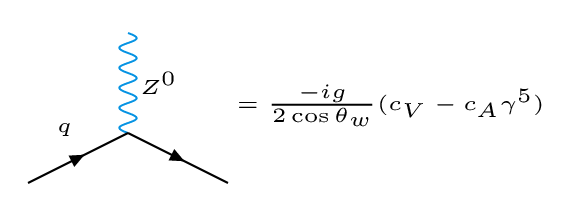
\includegraphics[width=0.7\linewidth]{figs/27a.png}
\newline
where for up-type quarks,
\begin{equation}
c_V = -\frac{4}{3}\sin^2\theta_w + \frac{1}{2}, \qquad c_A = \frac{1}{2};
\end{equation}
and for down-type quarks,
\begin{equation}
c_V = \frac{2}{3}\sin^2\theta_w - \frac{1}{2}, \qquad c_A = -\frac{1}{2}.
\end{equation}
%
\subsection{The GIM Mechanism - Glashow, Illiopoulos, Maiani (1970)}
%
For now let's consider only the light quarks $u$, $d$ and $s$. The down-type quarks are in general mixtures of the down-type components of the left-handed doublets. We can express this "Cabbibo mixing" using the Cabbibo angle $\theta_c$:
\begin{equation}
d^\prime = \cos\theta_c + \sin\theta_c.
\end{equation}
Then the neutral-current term $\bar{d}^\prime \gamma_\mu (c_V - c_A \gamma^5) d^\prime \equiv \bar{d}^\prime \Gamma d^\prime$, contains $\Delta Q = 0, \Delta S = 1$ pieces:
\begin{equation}
\sin\theta_c \cos\theta_c (\bar{d} \Gamma s + \bar{s} \Gamma d) .
\end{equation}
These are "flavour changing neutral currents" (FCNCs). The existence of these in the theory is embarrassing, because in actual fact $s \to d \nu \bar{\nu}$ never happens. There are experimental constraints set by Kaon decay rates:
\begin{equation}
\frac{\Gamma(K^+ \to \pi^+ \nu \bar{\nu})}{\Gamma(K^+ \to \text{all})} < 10^{-7}, \qquad \frac{\Gamma(K^0 \to \pi^+ \mu^+ \mu^-)}{\Gamma(K^0 \to \text{all})} < 10^{-8}.
\end{equation}
The solution is via the introduction of the charm quark, $c$. Then $\icol{c\\s^\prime}_L$ is an SU(2)$_L$ doublet, and if $s^\prime = -\sin\theta_L d + \cos \theta_c s$, the FCNCs cancel:
\begin{equation}
\bar{d}^\prime \Gamma d^\prime + \bar{s}^\prime \Gamma s^\prime =\bar{d} \Gamma d + \bar{s} \Gamma s.
\end{equation}
So with two generations (for three generations see later in the course), 
\[\left( \begin{array}{cc}
d^\prime \\
s^\prime 
\end{array} \right) =
 \left( \begin{array}{cc}
\cos\theta_c & \sin\theta_c \\
-\sin\theta_c & \cos\theta_c  \end{array} \right) 
\left( \begin{array}{cc}
d \\
s
\end{array} \right). \]
This predicted the existence of the charm quark, which was discovered in the form of the $J/\psi$ particle, a bound $c\bar{c}$ state of mass 3 GeV, in 1974 at SLAC/BNL.
%
\subsection{The Discovery of $W$ and $Z$}
%
The $W$ and $Z$ were discovered at SPS and CERN in 1983. They are easiest to produce in hadronic collisions.
\begin{figure}[!h]
  \centering
  \subfloat[$W$]{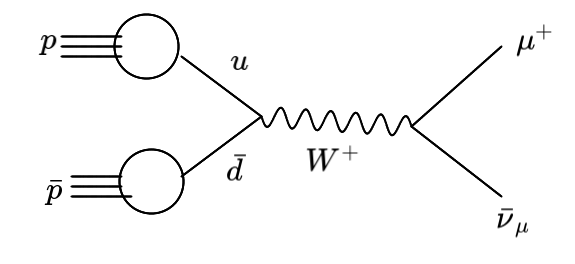
\includegraphics[width=0.4\textwidth]{figs/27b.png}}
  \hfill
  \subfloat[$Z$]{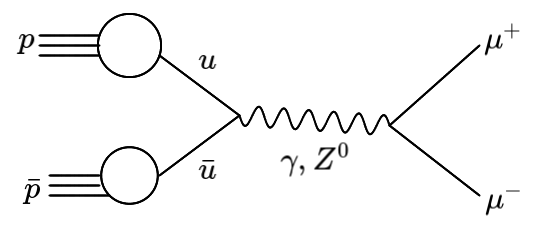
\includegraphics[width=0.4\textwidth]{figs/27c.png}}
\end{figure}
The partonic cross-sections are easy to calculate, allowing the properties of the $Z^0$ in particular to be explored with great precision at LEP (an $e^+ e^-$ collider operating from 1989-2001). This is because the $Z^0$ has a very clean final state signature, unlike the $W$ where the neutrino is not visible to the detectors. 
%
\newpage
%
\section{Spontaneous Symmetry Breaking and Mass (Weinberg, 1967)}
%
In summary of the situation thus far, the Lagrangian is made up of a $\psi$ kinetic term, a vector boson kinetic term, a $\psi$ mass term and a vector boson mass term:
\begin{equation}
\mathcal{L} = \mathcal{L}_D + \mathcal{L}_{YM} + \mathcal{L}_m + \mathcal{L}_M,
\end{equation}
where the first two terms are SU(2)$_L \otimes$U(1)$_Y$ gauge invariant, and the
second two break the symmetry: the problems are all to do with the mass terms.
\begin{equation}
\mathcal{L}_m = m(\bar{\psi}_L \psi_R + \bar{\psi}_R \psi_L) + ...
\end{equation}
breaks SU(2)$_L \otimes$U(1)$_Y$ explicitly, due to chirality, and
\begin{equation}
\mathcal{L}_M = m_W^2W_\mu^\dagger W^\mu + \frac{1}{2}m_Z^2 Z_\mu Z^\mu 
\end{equation}
also breaks SU(2)$_L \otimes$U(1)$_Y$ explicitly: $Z_\mu \neq W_\mu^3$ and $m_z \neq m_W$. We have Weinberg mixing, which again is due to chirality. 

Soft breaking of global symmetries is OK, but gauge symmetries must be exact so that the Noether current is conserved. Otherwise you miscount the degrees of freedom.
%
\subsection{Lepton Masses}
%
Under SU(2)$_L$:
\begin{equation}
\psi_L \to U \psi_L \qquad \text{and} \qquad \psi_R \to \psi_R, \qquad \text{where} \qquad U=\exp\bigg(\frac{i}{2}\underline{\alpha}\cdot\underline{\tau}\bigg);
\end{equation}
and under U(1)$_Y$:
\begin{equation}
\psi_L \to \exp\bigg(-\frac{i}{2}\beta\bigg) \psi_L \qquad \text{and} \qquad \psi_R \to \psi_R.
\end{equation}
An invariant mass term in SU(2)$_L \otimes$U(1)$_Y$ is impossible. But what about a Yukawa term ($\phi \bar{\psi} \psi$)? For this we need a scalar field, $\phi$. The simplest way to do this (but not the only way!) is to introduce a spin zero complex scalar doublet,
\[\phi = \left( \begin{array}{cc}
\phi^+ \\
\phi^0
\end{array} \right), \]
such that under SU(2)$_L$, $\phi \to U \phi$ (i.e. a doublet) and under U(1)$_Y$ $\phi \to \exp(i \beta /2)$ (i.e. $Y$ = 1/2). Then the additional Yukawa term in the Lagrangian looks like
\begin{equation}
\mathcal{L}_Y = -y_\psi(\bar{\psi}_L \phi \psi_R + \bar{\psi}_R \phi^\dagger \psi_L).
\end{equation}
This term is invariant because 
\begin{equation}
\bar{\psi}_L \phi \psi_R \to
\begin{cases}
\bar{\psi}_L U^\dagger U \phi \psi_R \qquad \qquad= \bar{\psi}_L \phi \psi_R \qquad \text{under SU(2)}_L,\\
\bar{\psi}_L e^{i \beta/2} e^{i \beta/2} \phi e^{-i\beta} \psi_R =\bar{\psi}_L \phi \psi_R \qquad \text{under U(1)}_Y.
\end{cases}
\end{equation}
Note that
\[ Q \qquad = \qquad T_3 \qquad + \qquad Y: \]
\[\left( \begin{array}{cc}
1 & 0  \\
0 & 0  \end{array} \right)=
\left( \begin{array}{cc}
1/2 & 0  \\
0 & -1/2  \end{array} \right) +
\left( \begin{array}{cc}
1/2 & 0  \\
0 & 1/2  \end{array} \right), \]
so $\phi^+$ has $Q = +1$ and $\phi^0$ has $Q=0$ (how fortuitous). Since $\phi^\dagger \phi$ is SU(2)$_L \otimes$U(1)$_Y$ invariant,
\begin{equation}
\mathcal{L}_\phi = \partial_\mu \phi^\dagger \partial^\mu \phi - V(\phi^\dagger \phi)
\end{equation}
has the correct global symmetry.

We still have no fermion masses. But because $\phi^0$ has $Q=0$ we can have spontaneous symmetry breaking. Choose a form for the potential
\begin{equation}
V(\phi^\dagger \phi) = \lambda \bigg(\phi^\dagger \phi - \frac{1}{2}v^2\bigg)^2.
\end{equation}
The minimum of $V$ is when $\phi^\dagger \phi = v^2/2$, so it's helpful to pick 
\[\phi^0 = \frac{1}{\sqrt{2}} = \left( \begin{array}{cc}
0   \\
v   \end{array} \right). \]
We can make this choice without loss of generality, due to global symmetry: we could have chosen e.g.
\[\phi^0 = u_0\frac{1}{\sqrt{2}} = \left( \begin{array}{cc}
0   \\
v   \end{array} \right), \]
but then let $\psi_L \to u_0 \psi_L$ and $\mathcal{W}_\mu \to u_0 \mathcal{W}_\mu u_0^\dagger$, and the Lagrangian would be unchanged.
Note that $i \underline{\alpha}\cdot \underline{T} \phi^0 \neq 0$, $i\beta\phi^0/2 \neq 0$, so both SU(2)$_L$ and U(1)$_Y$ are broken. But $Q\phi^0 = 0$ so U(1)$_Q$ remains unbroken. In other words SU(2)$_L$ $\otimes$U(1)$_Y$ $\to$ U(1)$_Q$. If we set $\phi \to \phi^0$ in $\mathcal{L}_Y$,
\begin{equation}
\mathcal{L}_Y \to -y_\psi (\bar{\psi}_L \phi_0 \psi_R + \bar{\psi_R} \phi_0^\dagger \psi_L) = -\frac{yv}{\sqrt{2}}(\bar{\psi}_L \psi_R + \bar{\psi}_R \psi_L) = -m_\psi \bar{\psi} \psi,
\end{equation}
i.e. we end up with the usual Dirac mass, where $m_\psi = y_\psi v/\sqrt{2}$, and is different for each of the leptons, dependent on their individual Yukawa couplings. The neutrinos remain massless. 

The only freedom is in the choice of $v$, which sets the scale, and in the parameters $y_e, y_\mu, y_\tau$ which fix the lepton masses.

Expanding around the minimum,
\[\phi = \phi^0 + \chi = \frac{1}{\sqrt{2}} \left( \begin{array}{cc}
\chi_1 + i \chi_2  \\
v + h + i \chi_3  \end{array} \right), \]
then 
\begin{equation}
\partial_\mu \phi^\dagger \partial^\mu \phi = \frac{1}{2} (\partial_\mu h)^2 + \frac{1}{2} (\partial_\mu \underline{\chi})^2, \qquad \text{where } \underline{\chi} = \chi_i; \ i=1,2,3.
\end{equation}
But
\begin{equation}
\phi^\dagger \phi -\frac{1}{2}v^2 = (\chi^\dagger \phi^0 + \phi^{\dagger 0}\chi) + \chi^\dagger \chi = vh + \frac{1}{2}h^2 + \frac{1}{2}\underline{\chi}^2,
\end{equation}
so 
\begin{equation}
V(\phi^\dagger \phi) = \lambda v^2 h^2 + \lambda v (h^3 + h \underline{\chi}^2) + \frac{\lambda}{4}(h^2 + \underline{\chi}^2)^2,
\end{equation}
so $h$ is massive: $m_h^2 = 2 \lambda v^2$, but the $\chi$ are massless: they are \textit{Goldstone} bosons. Because SU(2)$_L$ has dimension 3 and and U(1)$_Y$ and U(1)$_Q$ both have dimension 1, there are three Goldstone bosons because the degrees of freedom in the symmetry are reduced from 4 to 1 during symmetry breaking. $\lambda$ is a free parameter with a value $\approx 1/8$. 

Note that after spontaneous symmetry breaking we still have an SO(3) global symmetry, $\underline{\chi} \to R \underline{\chi}$, where $R^\dagger R =1$. This is called "custodial symmetry" or "custodial" SU(2) (because SO(3) $\cong$ SU(2)).

There are a number of vertices arising from the terms in $V$, which have the Feynman rules given in the figure.
\begin{figure}[!h]
  \centering
  \subfloat[3-point]{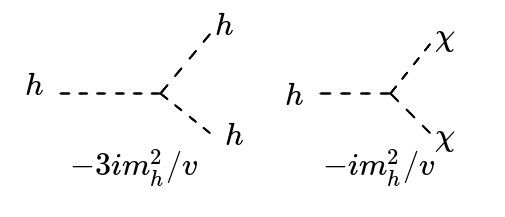
\includegraphics[width=0.5\textwidth]{figs/29a.png}}
  \hfill
  \subfloat[4-point]{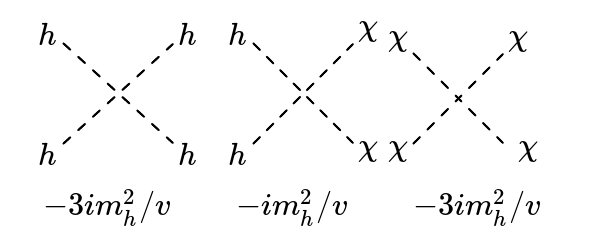
\includegraphics[width=0.5\textwidth]{figs/29b.png}}
\end{figure}
%
\subsection{Gauge Boson Masses}
%
$\mathcal{L}_\phi$ is invariant under \textit{global} SU(2)$_L \otimes$U(1)$_Y$. $\mathcal{L}_{YM}, \mathcal{L}_D$ and $\mathcal{L}_{Y}$ are all invariant under \textit{local} SU(2)$_L \otimes$U(1)$_Y$. So if we make $\mathcal{L}_\phi$ \textit{gauge} invariant, \textit{everything} will be gauge invariant! There is a unique prescription for achieving this:
\begin{equation}
\partial_\mu \phi \to \mathcal{D}_\mu \phi = (\partial_\mu - ig \mathcal{W}_\mu - \frac{1}{2} ig^\prime B_\mu) \phi,
\end{equation}
since $\phi$ is an SU(2) doublet, with $Y = +1/2$, and
\begin{equation}
\mathcal{L}_\phi \to \mathcal{L}_h = (\mathcal{D}_\mu \phi)^\dagger \mathcal{D}_\mu \phi - V(\phi^\dagger \phi).
\end{equation}
Now after spontaneous symmetry breaking, $\phi \to \phi^0 + \chi$, where $\partial_\mu \phi^0 = 0$. So
\begin{equation}
\begin{split}
\mathcal{D}_\mu \phi^0 &= -ig \underline{W}_\mu \cdot \underline{T}_\mu \phi^0 - \frac{1}{2} i g^\prime B_\mu \phi^0 \\
&= \frac{v}{2\sqrt{2}} 
\begin{pmatrix}  
-ig(W_\mu^1 - i W_\mu^2) \\
i(gW_\mu^3 - g^\prime B_\mu)
\end{pmatrix}, \\
\mathcal{D}_\mu \phi^{0 \dagger} \mathcal{D}^\mu \phi^0 &= \frac{v^2}{2} \bigg(\frac{g^2}{2} W_\mu^\dagger W^\mu + \frac{1}{4}(g W_\mu^3 - g^\prime B_\mu)^2 \bigg).
\end{split}
\end{equation}
So $m_W^2 = g^2v^2/4$, and $W$ becomes massive ($v \approx$ 50 GeV). $W_\mu^3$ and $B_\mu$ mix, but we know that already from the currents (because $j$ is not chiral).  
\[\left( \begin{array}{cc}
W^\mu_3 \\
B^\mu 
\end{array} \right) =
 \left( \begin{array}{cc}
\cos\theta_w & \sin\theta_w  \\
-\sin\theta_w & \cos\theta_w  \end{array} \right) 
\left( \begin{array}{cc}
Z^\mu \\
A^\mu 
\end{array} \right), \]
while $e = g \sin\theta_w = g^\prime \cos\theta_w$ so 
\begin{equation}
g W_\mu^3 - g^\prime B_\mu = \frac{g}{\cos \theta_w} (\cos\theta_w W_\mu^3 - \sin\theta_w B_\mu) = \frac{g}{\cos\theta} Z_\mu,
\end{equation}
and
\begin{equation}
\mathcal{D}_\mu \phi^{0 \dagger} \mathcal{D}^\mu \phi^0 = m_W^2 W_\mu^\dagger W^\mu + \frac{1}{2}m_Z^2 Z_\mu Z^\mu,
\end{equation}
with $m_Z^2 = g^2v^2/4\cos^2\theta_w = m_W^2/\cos^2\theta_w$, so $\rho = m_W^2/m_Z^2\cos^2\theta = 1$. $A_\mu$ remains massless, as expected, since U(1)$_Q$ is unbroken. So spontaneous symmetry breaking gives vector boson masses \textit{and} mixing.

There are also new interactions of vector bosons with scalars: $\phi = \phi^0 + \chi$, so
\begin{equation}
\mathcal{D}_\mu \phi^{\dagger} \mathcal{D}^\mu \phi = \mathcal{D}_\mu \phi^{0 \dagger} \mathcal{D}^\mu \phi^0 + \mathcal{D}_\mu \chi^{\dagger} \mathcal{D}^\mu \phi^0 + \mathcal{D}_\mu \phi^{0 \dagger} \mathcal{D}^\mu \chi + \mathcal{D}_\mu \chi^{\dagger} \mathcal{D}^\mu \chi,
\end{equation}
which leads to the mixing terms
\begin{equation}
ig(\phi^{0 \dagger} \underline{T} \partial_\mu \chi -\partial_\mu \chi^\dagger \underline{T} \phi^0) \cdot \underline{W}^\mu + i g^\prime (\phi^{0 \dagger} \partial_\mu \chi - \partial_\mu \chi^\dagger \phi^0) B^\mu.
\end{equation}
To simplify this, write $A_\mu^a = (W_\mu^i, B_\mu)$, $\tilde{T}^a = (gT^i, g^{\prime Y}) = (g\sigma^i/2, g^\prime/2)$, so that the mixing is
\begin{equation}
+i(\phi^{0 \dagger} \tilde{T}^a \partial_\mu \chi - \partial_\mu \chi^\dagger \tilde{T}^a \phi^0)A^{\mu a} = +i \tilde{J}_\mu^a A^{\mu a}.
\end{equation}
$\tilde{J}_\mu^a$ is actually the linear part of the Noether current of the SU(2)$_L \otimes$U(1)$_Y$ symmetry. In terms of real fields, writing 
\[\phi^0 = \frac{1}{\sqrt{2}} \left( \begin{array}{cc}
0 \\
v
\end{array} \right); \qquad
\chi = \frac{1}{\sqrt{2}}
 \left( \begin{array}{cc}
\chi_1 + i \chi_2 \\
h + i \chi_3  \end{array} \right), \]
it is easy to show (left as an exercise) that
\begin{equation}
\tilde{J}_\mu^a = -i F^{T a}_i \partial_\mu \chi_i = -i \partial_\mu \chi_i^T F_i^a,
\end{equation}
where
\[F_i^a = \frac{v}{2} \left( \begin{array}{cccc}
0 & -g & 0 & 0 \\
-g & 0 & 0 & 0 \\
0 & 0 & g & -g^\prime 
\end{array} \right). \]
So the mixing is between the vector bosons $A_\mu^a$ and the Goldstone bosons $\chi_i$ (\textit{not} the Higgs boson $h$): the mixing term is $A_\mu^a F^{a T} \partial_\mu \chi$. Note that
\begin{equation}
<0|\tilde{J}_\mu^a|\chi_i> = p_\mu F^a_i,
\end{equation}
so $F_i^a$ are the decay constants of the Goldstone bosons. $\partial^\mu \tilde{J}_\mu^a = 0 \implies p^2=0$ (i.e. the Goldstone bosons are massless: this is another derivation of Goldstone's theorem). It is easy to see that "$F^a = \tilde{T}^a \phi^0$ is the basis for the Goldstone bosons.

The mass term of the vector bosons is given by
\begin{equation}
\begin{split}
\mathcal{D}_\mu \phi^{0 \dagger} \mathcal{D}^\mu \phi^0 &= \frac{1}{2} \phi^{0 \dagger} \tilde{T}^a \tilde{T}^b \phi^0 A_\mu^a A^{\mu b} \\
&= \frac{1}{2}(F^TF)^{ab} A_\mu^a A^{\mu b}.
\end{split}
\end{equation}
In components,
\[(F^TF)^{ab} = \frac{v^2}{4} \left( \begin{array}{cccc}
g^2 & 0 & 0 & 0 \\
0 & g^2 & 0 & 0 \\
0 & 0 & g^2 & -gg^\prime \\
0 & 0 & - gg^\prime & g^{\prime 2} 
\end{array} \right), \]
with two $g^2v^2/4$ eigenvalues corresponding to $W^\pm$, one $(g^2 + g^{\prime 2})v^2/4$ eigenvalue corresponding to $Z$, and one $0$ eigenvalue corresponding to $\gamma$.

The equality of the first three diagonal elements is due to the SO(3) custodial symmetry, and ensures that the Veltman parameter
\begin{equation}
\rho = \frac{m_W^2}{m_Z^2 \cos^2\theta_w} = 1.
\end{equation}
%
\subsection{Unitarity Gauge}
%
As we now have a gauge theory, we need to fix a gauge (just as in QED): the degrees of freedom due to gauge transformations are not physical. One way to do this is to notice that the Goldstone bosons arise because of the SU(2)$_L \otimes$U(1)$_Y$ symmetry: for $\underline{\alpha}, \chi$ small, 
\begin{equation}
\begin{split}
&\text{SU(2)}_L: \quad U\phi \sim \phi^0 + i\underline{\alpha}\cdot \underline{T} \phi^0 + \chi = \frac{1}{\sqrt{2}} \bigg[ 
\begin{pmatrix}
0 \\ v
\end{pmatrix}
+ \frac{v}{2}
\begin{pmatrix}
(\alpha_2 + i \alpha_1) \\ -i\alpha_3
\end{pmatrix}
+ \begin{pmatrix}
\chi_1 + i \chi_2 \\ h + i \chi_3
\end{pmatrix} \bigg] \\
&\text{U(1)}_Y: \quad e^{i\beta /2}\phi \sim \phi^0 + i\frac{\beta}{2}\phi^0 + \chi = \frac{1}{\sqrt{2}} \bigg[ 
\begin{pmatrix}
0 \\ v
\end{pmatrix}
+ \frac{v}{2}
\begin{pmatrix}
0 \\ i\beta
\end{pmatrix}
+ \begin{pmatrix}
\chi_1 + i \chi_2 \\ h + i \chi_3
\end{pmatrix} \bigg],
\end{split}
\end{equation}
so we can eliminate $\chi_1, \chi_2, \chi_3$ just by choosing $\alpha_1, \alpha_2, \alpha_3, \beta$. Note that we cannot eliminate $h$: $\alpha_3 + \beta$ has no effect, since
\begin{equation}
Q \phi^0 = (T_3 + Y) \phi^0 = 0:
\end{equation}
U(1)$_Q$ is unbroken.

This is equivalent to adopting gauge fixing conditions for the broken symmetries:
\begin{equation}
\begin{split}
\chi^\dagger \underline{T} \phi^0 - \phi^{0 \dagger} \underline{T} \chi &= 0 \\
\chi^\dagger \phi^0 - \phi^{0 \dagger} \chi &= 0,
\end{split}
\end{equation}
i.e. $F_i^T\chi_i=0 \implies \chi_i=0$. With these conditions, the mixing terms between vector bosons and Goldstone bosons disappear, and we can write
\[\phi = \frac{1}{\sqrt{2}} = \left( \begin{array}{cc}
0   \\
v + h  \end{array} \right). \]
Substituting into the Lagrangian, 
\end{document}